\PassOptionsToPackage{unicode=true}{hyperref} % options for packages loaded elsewhere
\PassOptionsToPackage{hyphens}{url}
%

\documentclass[11pt,openany]{book}
% \usepackage[dvipsnames,svgnames*,x11names*]{xcolor}
\usepackage[svgnames]{xcolor}
\usepackage{titlesec}
\usepackage{graphicx}
% \usepackage{lipsum}
\usepackage[all]{nowidow}
\usepackage[none]{hyphenat}
\usepackage{pdflscape}

\usepackage{fontspec}
\usepackage{xunicode}
\usepackage{xltxtra}

  \setmainfont{Bookerly}
  \setsansfont{Oswald}
  \setmonofont{Source Sans Pro}
\usepackage{sectsty}
\allsectionsfont{\sffamily}

% Dates
%-------
\usepackage{datetime}
\newdateformat{yearonly}{\THEYEAR}
\newdateformat{usmonthyear}{\monthname[\THEMONTH], \THEYEAR}
\newcommand{\monthyear}{%
  \ifcase\month\or January\or February\or March\or April\or May\or June\or
  July\or August\or September\or October\or November\or
  December\fi\space\number\year
}

\usepackage{amssymb,amsmath}
\usepackage{ifxetex,ifluatex}
\usepackage{fixltx2e} % provides \textsubscript
\ifnum 0\ifxetex 1\fi\ifluatex 1\fi=0 % if pdftex
  \usepackage[T1]{fontenc}
  \usepackage[utf8]{inputenc}
  \usepackage{textcomp} % provides euro and other symbols
\else % if luatex or xelatex
  \usepackage{unicode-math}
  \defaultfontfeatures{Ligatures=TeX,Scale=MatchLowercase}
\fi
% use upquote if available, for straight quotes in verbatim environments
\IfFileExists{upquote.sty}{\usepackage{upquote}}{}
% use microtype if available
\IfFileExists{microtype.sty}{%
\usepackage[]{microtype}
\UseMicrotypeSet[protrusion]{basicmath} % disable protrusion for tt fonts
}{}
\IfFileExists{parskip.sty}{%
\usepackage{parskip}
}{% else
\setlength{\parindent}{0pt}
\setlength{\parskip}{6pt plus 2pt minus 1pt}
}
\usepackage{hyperref}
\hypersetup{
            pdftitle={Verkilo Business Plan},
            pdfauthor={Birchfield, Koprowski, Wilson},
            pdfborder={0 0 0},
            breaklinks=true}
\urlstyle{same}  % don't use monospace font for urls

\newcommand{\AFourSize}{ paperwidth=21.00cm,paperheight=29.70cm,margin=20mm,twoside}
\newcommand{\Letter}{    paperwidth=21.59cm,paperheight=27.94cm,margin=25mm,twoside}                              % 8.5x11"
\newcommand{\LargeTrade}{paperwidth=20.32cm,paperheight=25.40cm,outer=17mm,bottom=17mm,top=2cm,inner=2cm,twoside} % 8x10"
\newcommand{\Textbook}{  paperwidth=17.78cm,paperheight=25.40cm,outer=17mm,bottom=17mm,top=2cm,inner=2cm,twoside} % 7x10"
\newcommand{\Trade}{     paperwidth=15.24cm,paperheight=22.86cm,outer=17mm,bottom=17mm,top=2cm,inner=2cm,twoside} % 6x9"
\newcommand{\Digest}{    paperwidth=13.97cm,paperheight=21.59cm,outer=17mm,bottom=17mm,top=2cm,inner=2cm,twoside} % 5.50x8.5"
\newcommand{\SmallTrade}{paperwidth=13.34cm,paperheight=20.32cm,outer=13mm,bottom=17mm,top=2cm,inner=2cm,twoside} % 5.25x8"
\newcommand{\Novella}{   paperwidth=12.70cm,paperheight=20.32cm,outer=13mm,bottom=17mm,top=2cm,inner=2cm,twoside} % 5x8"
\newcommand{\UKBFormat}{ paperwidth=12.90cm,paperheight=19.80cm,outer=17mm,bottom=17mm,top=2cm,inner=2cm,twoside}
\newcommand{\UKAFormat}{ paperwidth=11.10cm,paperheight=17.80cm,outer=17mm,bottom=17mm,top=2cm,inner=2cm,twoside}
\newcommand{\AFourSizeLinespace}{ 1.4}
\newcommand{\LetterLinespace}{    1.4} % 11"
\newcommand{\LargeTradeLinespace}{1.4} % 10"
\newcommand{\TextbookLinespace}{  1.4} % 10"
\newcommand{\TradeLinespace}{     1.2} % 9"
\newcommand{\DigestLinespace}{    1.1}
\newcommand{\SmallTradeLinespace}{1.1}
\newcommand{\NovellaLinespace}{   1.1}
\newcommand{\UKBFormatLinespace}{ 1.1}
\newcommand{\UKAFormatLinespace}{ 1.1}


% \newcommand{\AFourSize}{ paperwidth=210mm, paperheight=297mm,margin=2cm,twoside}
% \newcommand{\Letter}{    paperwidth=8.50in,paperheight=11in, margin=1.0in,twoside}
% \newcommand{\LargeTrade}{paperwidth=8.00in,paperheight=10in, left=0.875in,outer=0.825in,top=0.825in,bottom=0.825in,twoside}
% \newcommand{\USTextbook}{paperwidth=7.00in,paperheight=10in, left=0.875in,outer=0.825in,top=0.825in,bottom=0.825in,twoside}
% \newcommand{\Trade}{     paperwidth=6.00in,paperheight=9in,  left=0.875in,right=0.625in,top=0.525in,bottom=0.625in,twoside}
% \newcommand{\Digest}{    paperwidth=5.50in,paperheight=8.5in,left=0.875in,right=0.625in,top=0.825in,bottom=0.625in,twoside}
% \newcommand{\SmallTrade}{paperwidth=5.25in,paperheight=8in,  left=0.875in,right=0.625in,top=0.825in,bottom=0.625in,twoside}
% \newcommand{\Novella}{   paperwidth=5.00in,paperheight=8in,  left=0.775in,right=0.525in,top=0.825in,bottom=0.625in,twoside}
% \newcommand{\MassMarket}{paperwidth=4.25in,paperheight=7in,  left=0.775in,right=0.525in,top=0.825in,bottom=0.625in,twoside}
% \newcommand{\UKAFormat}{ paperwidth=111mm, paperheight=178mm,left=2cm,right=15mm,top=2cm,bottom=16mm,twoside}
% \newcommand{\UKBFormat}{ paperwidth=129mm, paperheight=198mm,left=2cm,right=15mm,top=2cm,bottom=16mm,twoside}
\usepackage[\Letter]{geometry}

\usepackage{setspace}
\setstretch{1.6}


\usepackage{longtable,booktabs}
% Fix footnotes in tables (requires footnote package)
\IfFileExists{footnote.sty}{\usepackage{footnote}\makesavenoteenv{longtable}}{}
\usepackage{graphicx,grffile}
\makeatletter
\def\maxwidth{\ifdim\Gin@nat@width>\linewidth\linewidth\else\Gin@nat@width\fi}
\def\maxheight{\ifdim\Gin@nat@height>\textheight\textheight\else\Gin@nat@height\fi}
\makeatother
% Scale images if necessary, so that they will not overflow the page
% margins by default, and it is still possible to overwrite the defaults
% using explicit options in \includegraphics[width, height, ...]{}
\setkeys{Gin}{width=\maxwidth,height=\maxheight,keepaspectratio}
\setlength{\emergencystretch}{3em}  % prevent overfull lines
\providecommand{\tightlist}{%
  \setlength{\itemsep}{0pt}\setlength{\parskip}{0pt}}
\setcounter{secnumdepth}{0}
% Redefines (sub)paragraphs to behave more like sections
\ifx\paragraph\undefined\else
\let\oldparagraph\paragraph
\renewcommand{\paragraph}[1]{\oldparagraph{#1}\mbox{}}
\fi
\ifx\subparagraph\undefined\else
\let\oldsubparagraph\subparagraph
\renewcommand{\subparagraph}[1]{\oldsubparagraph{#1}\mbox{}}
\fi

% set default figure placement to htbp
\makeatletter
\def\fps@figure{htbp}
\makeatother
\titleformat{\chapter}[display]
  {\normalfont\sffamily\Large\color{Black}}
  {}{0pt}{\Huge}

\newcommand{\hideFromPandoc}[1]{#1}
\usepackage{pdflscape}
\usepackage{lscape}
\usepackage{scrextend}
 \let\Begin\begin \let\End\end 
\usepackage{xcolor}
\titlespacing*{\chapter}{0pt}{1cm}{1cm}
\usepackage{spreadtab}
\definecolor{red}{cmyk}{0.0, 0.56, 0.43, 0.58}
\definecolor{blue}{cmyk}{0.56, 0.21, 0, 0.58}
\definecolor{yellow}{cmyk}{0, 0.0, 0.56, 0.58}
\definecolor{orange}{cmyk}{0, 0.34, 0.56, 0.58}
\usepackage{lipsum}
\setmonofont{Source Sans Pro}
\usepackage{adjustbox}
% HEADER DESIGN
\usepackage{fancyhdr} % headers
\pagestyle{fancy} % style for headers
\usepackage{pifont} % for the copyright symbol
\headheight 0.25in % height of header
\headsep 0.25in % dist between top of text and bottom of header
\parskip 0in
\parindent 0.25in % = 6.35mm
\newcommand{\str}{\rule{0pt}{16pt}} % strut used in toc
%%% header stuff
\newcommand{\currpage}{\footnotesize\thepage} % use in headers
\fancyhead{} % clear header fields, required
\fancyfoot{} % clear footer fields, required
% \fancyfoot[C]{\currpage}
\fancyhead[LE,RO]{\currpage}

\fancyhead[CO]{ \footnotesize\MakeUppercase{Verkilo Business
Plan}  } % Odd Page, Right side
\fancyhead[CE]{ \footnotesize\MakeUppercase{Birchfield, Koprowski,
Wilson} } % Even Page, Right side
\renewcommand\headrulewidth{0pt} % for no rule line under header

  % \titleformat{\chapter}[display]
    % {\normalfont\sffamily\huge\bfseries\color{Black}}
    % {\chaptertitlename\ \thechapter}{20pt}{\Huge}
% \titleformat{\chapter}[display]
%   {\bfseries\Large}
%   {\filright\MakeUppercase{\chaptertitlename} \Huge\thechapter}
%   {1ex}
%   {\titlerule\vspace{1ex}\filleft}
%   [\vspace{1ex}\titlerule]

\newlength{\cslhangindent}
\setlength{\cslhangindent}{1.5em}
\newenvironment{cslreferences}%
  {\setlength{\parindent}{0pt}%
  \everypar{\setlength{\hangindent}{\cslhangindent}}\ignorespaces}%
  {\par}
% ===============================================
% Bringing PlainFancyBreak from Memoir class.
\makeatletter
\newcommand{\plainfancybreak}{\@ifstar{\@spfbreak}{\@pfbreak}}
\newcommand{\@pfbreak}[3]{\par
  \@tempdimc\pagegoal \advance\@tempdimc-\pagetotal
  \ifdim #1>\@tempdimc \@fbreak{#3}\else \@pbreak{#2}\fi}
\newcommand{\@spfbreak}[3]{\par
  \@tempdimc\pagegoal \advance\@tempdimc-\pagetotal
  \ifdim #1>\@tempdimc \@sfbreak{#3}\else \@spbreak{#2}\fi}

\newcommand*{\pen@ltyabovepfbreak}{2}
\newcommand*{\pen@ltybelowpfbreak}{-4}

\newlength{\pfbreakskip}
  \setlength{\pfbreakskip}{2\baselineskip}
\newcommand{\pfbreakdisplay}{*\quad*\quad*}

\def\pfbre@kdispl@y{\vbox to 1\pfbreakskip{\vss
  \hb@xt@ \columnwidth{\hss \pfbreakdisplay \hss}%
  \vss}}

\edef\nopfbreakOutput{\the\output}
\def\pfbreakOutput{%
  \ifnum\outputpenalty=\pen@ltyabovepfbreak
    \nopfbreakOutput
    \pfbre@kdispl@y
    \nobreak
    \vskip-\pfbreakskip
  \else\ifnum\outputpenalty=\pen@ltybelowpfbreak
    \unvbox 255\relax
    \nobreak
    \vskip-\pfbreakskip
    \pfbre@kdispl@y
    \break
  \else
    \nopfbreakOutput
  \fi
  \fi}
\output={\pfbreakOutput}

\newcommand{\pfbreak}{\@ifstar{\@spfbreakgap}{\@pfbreakgap}}
\newcommand{\@pfbreakgap}{%
  \par {%
  \skip@\lastskip
  \nobreak
  \vskip -\ifdim\prevdepth>\maxdepth \maxdepth
          \else\ifdim\prevdepth>-1000pt\prevdepth
            \else\ifinner 0pt
              \else \pagedepth
          \fi \fi \fi
  \vskip -\skip@
  \ifdim\skip@<\pfbreakskip
    \advance\skip@ -1\skip@ \advance\skip@ 1\pfbreakskip
  \fi
  \penalty\pen@ltyabovepfbreak
  \vskip\skip@
  \penalty\pen@ltybelowpfbreak
  }
  \@afterindentfalse
  \@afterheading
}
\newcommand{\@spfbreakgap}{%
  \par {%
  \skip@\lastskip
  \nobreak
  \vskip -\ifdim\prevdepth>\maxdepth \maxdepth
          \else\ifdim\prevdepth>-1000pt\prevdepth
            \else\ifinner 0pt
              \else \pagedepth
          \fi \fi \fi
  \vskip -\skip@
  \ifdim\skip@<\pfbreakskip
    \advance\skip@ -1\skip@ \advance\skip@ 1\pfbreakskip
  \fi
  \penalty\pen@ltyabovepfbreak
  \vskip\skip@
  \penalty\pen@ltybelowpfbreak
  }
  \@afterindenttrue
  \@afterheading
}
\makeatother
% /PlainFancyBreak
\counterwithout{figure}{chapter}
\counterwithout{table}{chapter}
\begin{document}
  \sloppy % ignore problems with line overflow / underflow
  \setcounter{page}{1}
% ===============================================
% Old Beamer frontmatter
% %   %     % \maketitle
%   %   % 
% ===============================================
% Frontmatter
  \pagenumbering{roman}
  \pagestyle{empty}
  % ------------------------------------------------
  % r.1 - Half-Title - Recto
  \begin{center}
    \vspace*{\fill}

    \LARGE\textbf{\textsf{Verkilo Business Plan}}

    \vspace*{\fill}
    \vspace*{\fill}
  \end{center}
  \clearpage

  % ------------------------------------------------
  % r.2 - Series Title Page - Verso
  \newpage
  \emph{ }\newline
    \clearpage

  % ------------------------------------------------
  % r.3 Titlepage - Recto
  \begin{center}
    \vspace*{\fill}

    \Huge\textbf{\textsf{Verkilo Business Plan}}
    
    \vspace*{0.125in}
    \Large\textbf{\textsf{Helping Authors Manage Their Creativity}}
    
    \vspace*{0.25in}
    \line(1,0){150}
    \vspace*{0.25in}

    \Large\textsf{Birchfield, Koprowski, Wilson}

    \vspace*{\fill}
    \vspace*{\fill}
      \end{center}
  \clearpage

  % ------------------------------------------------
  % r.4 Copyright Page
  \vspace*{\fill}

  \par\noindent\emph{Verkilo Business Plan}\newline
  \par\noindent\emph{Copyright © 2020 Bryan Birchfield, Robert
Koprowski, Ben Wilson}\newline

  \footnotesize
  \par\noindent No part of this publication may be reproduced, stored in
a retrieval system, posted on the Internet, or transmitted, in any form
or by any means, electronic, mechanical, photocopying, recording, or
otherwise, without prior written permission from the authors. The only
exception is by a reviewer, who may quote short excerpts in a
review.\newline


  \footnotesize
  

  % Producer Acknowledgements
  \par\noindent Interior Design: Merovex Press % Per license terms for use of template.
      \par\noindent Formatting: This document was formatted using
Verkilo's prototype Formatter
      \par\noindent Editor: Cynthia Shepp
  \newline

  \par\noindent       \par\noindent Birchfield, Koprowski, Wilson
    \newline

  
  \par\noindent Printed in the United States of America
  \newline

  
    \par\noindent Version: v0.1
    \vspace*{\fill}
  \clearpage\normalsize

  % -----------------------------------------------
  % r.5 - Dedication
  
  % -----------------------------------------------
  % Table of Contents
              {
            \makeatletter
      \renewcommand*\l@section{\@dottedtocline{1}{1.5em}{3.0em}}
      \makeatother
      \setcounter{tocdepth}{2}
      \tableofcontents
    }
      
  % -----------------------------------------------
  % List of Tables
      \listoftables
  
  % -----------------------------------------------
  % List of Figures
      \listoffigures
  
\newpage % End Frontmatter

% ===============================================
% Mainmatter
\pagenumbering{arabic}\pagestyle{fancy}
\chapter{Executive Summary}

Traditional publishing offers a professional workflow that helps authors
turn their creations into publishable products. The publishing field is
competitive, resulting in a high author-rejection rate. The
self-publishing market comprises one-third of the US publishing market,
representing \$9.1 billion of the \$26 billion in gross US annual book
revenue.

The quality of self-published titles is lower than traditional
publishing due in part to a lack of professional editing, which, in
turn, leads to a growing market of freelance editors. Authors and
editors alike are challenged with finding a suitable counterpart who can
work within their schedule. Editors are especially frustrated by authors
with unrealistic expectations, which leads to lower quality-of-life and
burnout in the editing community.

Verkilo seeks to streamline the self-published author workflow through a
two-sided platform where authors create their work and are automatically
paired with a suitable editor for final collaboration. This will reduce
friction in the production process for the author, and by assisting with
scheduling we will improve our editor's quality of life. As a platform,
we are like Airbnb and Uber. We generate revenue in two ways: by levying
a service charge on author/editor transactions and by charging a monthly
subscription to the authors. By establishing a modest foothold in the
self-publishing industry by Year 5, we expect to generate \$4.5 million
in revenue. Our ideal exit strategy is acquisition by Amazon.

No unified, two-sided platform exists in the publishing industry that
offers automated author/editor pairing with content creation and
automated formatting. Most content creation and editing occur in
standalone products like Microsoft Word and Google Docs. Existing
pairing platforms like Reedsy rely on manual pairing. Other products in
the industry focus on niche aspects such as formatting.

We seek \$1.2 million in seed money for 20\% in equity so we can beat
rivals to market and establish a strong brand presence. Verkilo will use
seed funding to finance its first steps, including refined market
research and product development. With seed funding, Verkilo can
determine what its final products will be and who its target demographic
is. We will use seed funding to employ a founding team to complete these
tasks. We estimate the rate of return for this investment in Year 5 will
be \$13.2 million.

\hypertarget{value-proposition}{%
\chapter{Value Proposition}\label{value-proposition}}

\hypertarget{vision}{%
\section{Vision}\label{vision}}

Verkilo will create a fully integrated, content-creation platform to
help self-published authors create professional-grade books by
automatically pairing the author with available freelance editors using
a machine-learning matchmaking algorithm. Self-published authors need to
work with their supporting editor on a schedule that supports the
author's targeted release date and the editor's hectic schedule. Verkilo
is an application that works on any device wherever the author and
editor are comfortable. Verkilo's unique value proposition removes
friction from author and editor by automating the production process.
This taps into a multibillion-dollar industry in need of optimization.

Verkilo will build a cutting edge, technology-based platform that
professionals in the self-publishing market will recognize as the leader
in their community. This platform will support and enhance the delivery
and time to market of professional-grade, self-published literature.
Company primary revenue will be generated by a service charge processed
against each editorial transaction conducted by the respective editors.
Verkilo will develop and market its own product offering that leverages
the agility of cloud technology and dynamically enhanced through
data-drive machine learning for speed to market.

\newpage

\hypertarget{business-problem}{%
\section{Business Problem}\label{business-problem}}

The publishing industry is undergoing tremendous transformation where
traditional media is being displaced by self-published authors. This
leads to a problem where the author, as creator, must also fill the role
of product manager. The author must plan and execute all aspects of
production from finding and scheduling editors and cover artists to
formatting the final copy and handling distribution and marketing. This
steals precious time and energy from the author's core role as the
creative artist.

Likewise, freelance editors are frustrated by the challenges of
scheduling and coordinating their work. They work directly with authors
who are unfamiliar with the traditional publishing process and find
themselves frequently managing authors' unrealistic schedule
expectations and lack of professional discipline ---often submitting
manuscripts late and changing a draft after it has been submitted. This
contention results in work-life balance complaints among freelance
editors and tends to produce lower-quality self-published books released
to market. Authors and editors would rather focus on their respective
specialties and not contend with the hassles of coordinating their work
with one another. By creating the solution through Verkilo's offerings,
we help self-published authors work more collaboratively with freelance
editors on the editors' timetable. Our goal here at Verkilo is to
improve the quality of self-published books for global consumption in
addition to providing a balanced work-life for editors, thus increasing
earnings for both author and editor alike.

\hypertarget{solution}{%
\section{Solution}\label{solution}}

Verkilo helps authors and editors create professional, publishable books
without all the hassles. We create a collaborative platform where
authors and editors can work anywhere, any time by offering a
cross-device application (web, Windows, MacOS, iOS, Android, plugins).
Verkilo monitors the author's progress and creates a production schedule
with editors who have similar audience and genre interests, and who are
available to edit when the book is projected to be ready. When the
author is ready to distribute, the book is professionally formatted into
industry-standard file formats (ePUB, PDF). As 80\% of self-published
authors use Amazon's Kindle Direct Publishing (KDP), these formats are
perfect for uploading directly to KDP for sale on Amazon.

Sequoia Capital, an American venture capital firm, describes American
Express, PayPal, eBay, Uber, Facebook, WhatsApp, Netflix, and Amazon all
as two-sided platforms. (Sequoia, 2018) These platforms exist as
intermediaries to match the supply and demand sides of a market
efficiently. Verkilo endeavors to provides a similar two-sided
marketplace for editors and authors to collaborate.

Verkilo helps authors and editors create professional, publishable books
without all the hassles. We create a collaborative platform where
authors and editors can work anywhere, any time by offering a
cross-device application (web, Windows, MacOS, iOS, Android, plugins).

\hypertarget{validation}{%
\section{Validation}\label{validation}}

As discussed in the above Business Problem and Solution sections, market
research analysis was completed through web crawling public forums,
blogs, and community websites. This includes Reddit's r/self-publish
channel comprising 36,700 members (\emph{Self Published Writers}, n.d.)
and the 20BooksTo50K® Facebook group comprising 35,800 members.
(\emph{20BooksTo50K®}, n.d.) We conducted an online survey of likely
self-published editors via direct Facebook advertisement over a period
of two weeks. This market research supported our assumption and
suggested baseline requirements to support self-published authors and
freelance editors in our target audience. Surveyed editors described
their biggest challenge was finding suitable authors who matched their
desired genre of editing that had realistic expectations to work within
an editor's schedule. These challenges directly affect the editors'
quality of life, contribute to their daily frustration, and diminish the
overall professional relationship with authors.

\hypertarget{market-analysis}{%
\chapter{Market Analysis}\label{market-analysis}}

Verkilo initially targets US self-published authors and editors. As
discussed below, the US self-publisher market is one-third of the total
US published market (itself a quarter of the global market) and is
displacing traditional publishing. The overall market should grow
modestly for the foreseeable future, with US self-publishers potentially
grossing between \$9 and \$28 billion in annual revenue by 2025. Our
market landscape analysis reflects a diverse market of products and
services that compete with Verkilo's vision for attention in the
self-publisher market. However, our quantitative assessment suggests
none are competing against our complete vision for hassle-free
self-publishing.

Verkilo initially plans to target the highly valuable US self-publishing
community. The US self-publisher market is one-third of the total US
published market (itself a quarter of the global market) and is
displacing traditional publishing. The overall market shows considerable
growth for the foreseeable future, with estimates grossing between \$9
and \$28 billion in annual revenue by 2025 for US self-publishers. Our
market landscape analysis reflects a diverse market of products and
services currently available that compete with Verkilo's vision for
attention in the self-publisher market. However, our quantitative
assessment suggests none are competing against our vision of a complete
vertical integration of software product offering for hassle-free
self-publishing managed through machine learning

\newpage

\hypertarget{market-size}{%
\section{Market Size}\label{market-size}}

The US book-publishing industry generated \$28 billion in annual revenue
in 2018. (Watson, 2019) This represents 23\% of the \$119 billion in
global annual revenue. (\emph{Global Book Publishing Industry Outlook},
2019) US self-published authors represent 35\% of the US market, valued
at \$7.8 billion.

Bowker, the US registrar for ISBNs (International Standard Book Number),
reported 1.6 million books published by self-published authors in 2018,
including 490,000 new self-published titles released in 2018 with an
assigned ISBN.\footnote{Bowker warned many books in 2018 distributed via
  Amazon's Kindle without ISBNs, which means the total number of
  self-published books exceeds the Bowker reported number.
  (``Self-Publishing in the United States, 2013-2018 Print and Ebooks,''
  2019) We limited our analysis to verifiable numbers provided by
  Bowker.} (\emph{Self-Publishing Grew 40 Percent in 2018, New Report
Reveals}, 2019) From 2010 to 2018, the number of self-published book
titles increased an average of 30\% each year. (``Self-Publishing in the
United States, 2013-2018 Print and Ebooks,'' 2019) As the overall US
market publishing market grew at a slower pace, this increase represents
a displacement of traditional publishing by self-publishers. Forbes
reported there were three self-published books for every traditionally
published book as of 2017. (Pofeldt, 2019) Eighty-five percent of
self-published books with ISBNs from 2013 to 2018---or 1.4 million
titles---were distributed via Amazon's Kindle Direct Published
Publishing (KDP), which replaced Amazon's CreateSpace.
(``Self-Publishing in the United States, 2013-2018 Print and Ebooks,''
2019)

\begin{figure}
\centering
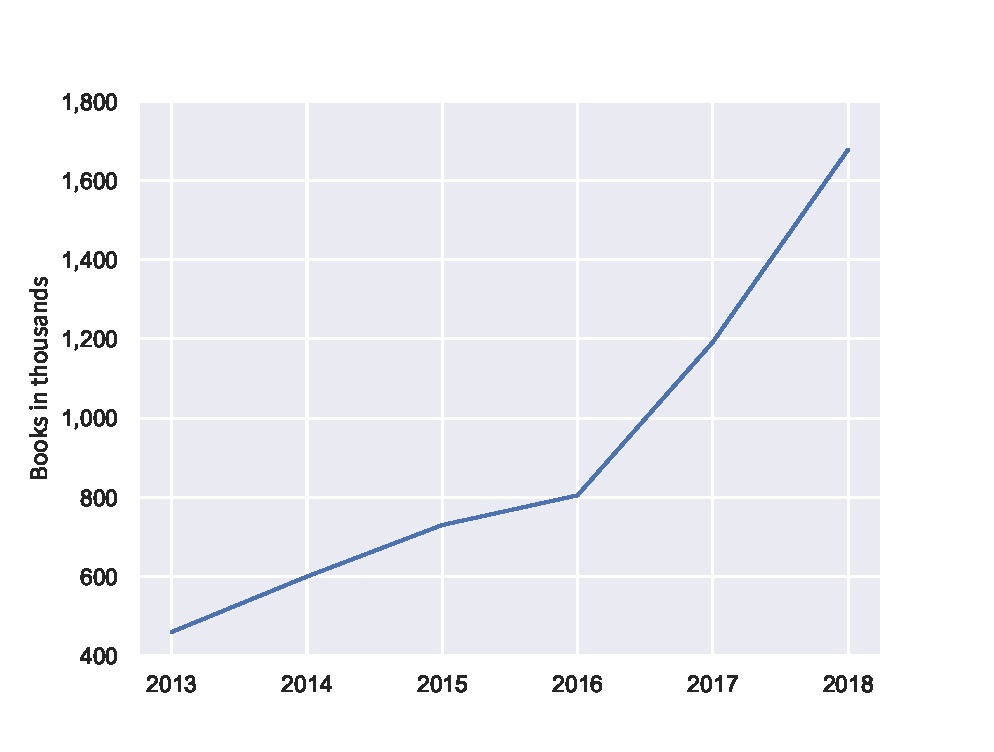
\includegraphics{media/book-sales.eps}
\caption{Self-Published Books with ISBNs 2013-2018}
\end{figure}

Technavio, a leading global technology research and advisory company,
estimates the global publishing market size will grow by \$23 billion to
\$142 billion between 2020-2024; a 19\% increase over the next four
years or 6\% each year. (``Publishing Market by Platform and Geography -
Forecast and Analysis 2020-2024,'' 2019) The US market should grow at a
similar pace to \$33 billion. If US self-publishing grows at the same
rate (instead of its historic 30\% rate), its market size may reach \$11
billion by 2024. At 6\% annual growth from Bowker's 2018 numbers, we
estimate a total of 3.8 million self-published books will be released
between 2020 and 2025. (``Self-Publishing in the United States,
2013-2018 Print and Ebooks,'' 2019)

\begin{figure}
\centering
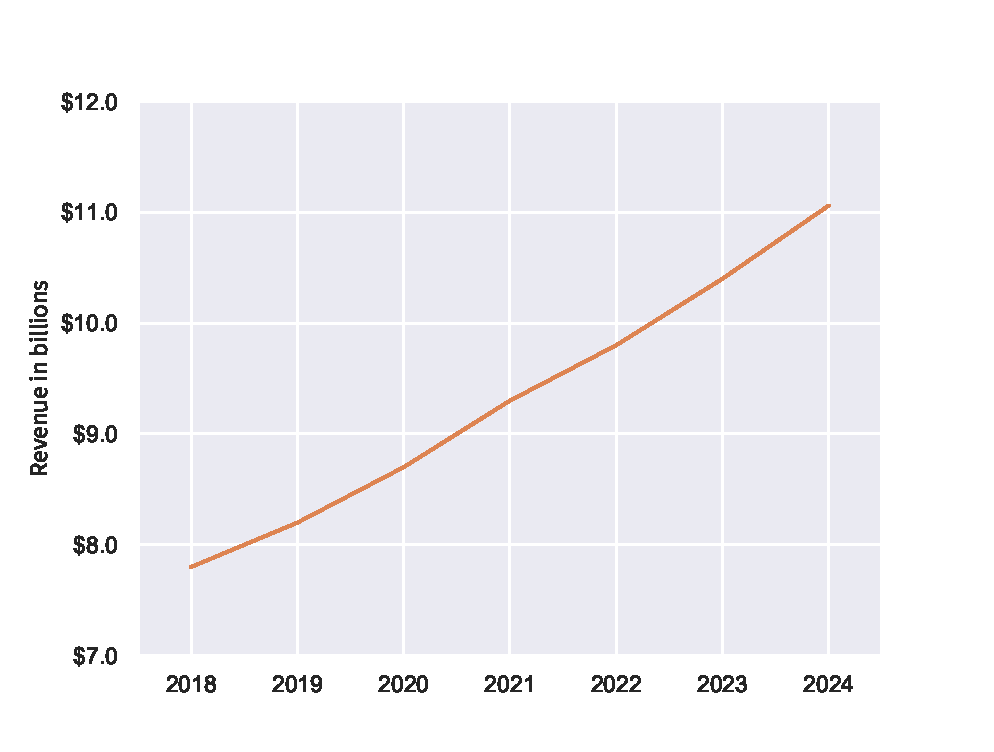
\includegraphics{media/market-growth.eps}
\caption{Forecasted Annual Growth of Self-Published Market 2020-2024}
\end{figure}

\newpage

\hypertarget{market-landscape}{%
\section{Market Landscape}\label{market-landscape}}

Our market landscape analysis shows a diverse market of products and
services that compete with Verkilo's vision. Our market assessment
aligns with Porter's Five Forces as applied to software as a service
(SaaS). (Niebauer, 2018) The competitive nature of this segment requires
we establish brand and product differentiation to stand out. Verkilo
seeks to compete by having a complete, compelling vision of the
production cycle and automating processes the competition leaves manual.

\textbf{New Entrant Threat---High.} The threat of new entrants in any
SaaS-related market is high because the ease of establishing
infrastructure and product is low.

\textbf{Supplier Bargaining Power---Low.} Suppliers such as
infrastructure providers have limited bargaining power due to the
presence of many infrastructure and platform providers that have
commoditized storage, computers, databases, and other services. Supplier
costs are a small proportion of any SaaS company's expenses. (Niebauer,
2018)

\textbf{Buyer Bargaining Power---Very High.} The competitive nature of
SaaS markets results in companies giving significant information to the
customer in the form of pre-sales information, free trials, and
low-commitment, monthly rollover contracts. To compete, Verkilo must
establish brand loyalty and drive long-term value for the customer.

\textbf{Substitute Product Threat / Competitive Rivalry---Very High.}
SaaS companies like Verkilo live and die by product differentiation,
which creates fierce competitive rivalry as customers have comparably
low switching costs. (Niebauer, 2018) We focus on competition in the
following section due to our need to differentiate .

\newpage

\hypertarget{competition}{%
\section{Competition}\label{competition}}

To measure the market landscape, we leverage Gartner's methodology to
quantitatively assess the market landscape. (``Magic Quadrant Research
Methodology,'' 2020) Verkilo views four criteria essential in defining a
complete vision for a self-publisher's platform. We measured each on a
5-point Likert scale and averaged the result results to get a vision
index.

\hypertarget{vision-criteria-for-a-self-publishers-platform}{%
\subsubsection{Vision Criteria for a Self-Publishers
Platform}\label{vision-criteria-for-a-self-publishers-platform}}

\begin{enumerate}
\def\labelenumi{\arabic{enumi}.}
\tightlist
\item
  \textbf{Complex Document Project Management.} Enables the
  self-published author to manage complex and interrelated documents (an
  entire fiction series or milieu for example)
\item
  \textbf{Intelligent Matchmaking.} Advances machine learning in
  automating the identification and collaboration of book-publishing
  professionals
\item
  \textbf{Professional Final Product.} Delivers a final product that is
  indistinguishable from traditionally published products
\item
  \textbf{Learning Community.} Draws self-published authors together to
  enhance the writing community and provide fine literature
\item
  \textbf{User Experience.} Overall experience using the product,
  including how easy or pleasing it is to use.
\end{enumerate}

The table below lists the top products in the self-publishing market
that support content creation, revision, publication, or community. TBD-
Appendix explaining why we scored each

\newpage

\begin{longtable}[]{@{}lcccccc@{}}
\caption{Assessment of Completeness of Competitors'
Vision}\tabularnewline
\toprule
\begin{minipage}[b]{0.29\columnwidth}\raggedright
Product\strut
\end{minipage} & \begin{minipage}[b]{0.09\columnwidth}\centering
Manage\strut
\end{minipage} & \begin{minipage}[b]{0.08\columnwidth}\centering
Match\strut
\end{minipage} & \begin{minipage}[b]{0.09\columnwidth}\centering
Output\strut
\end{minipage} & \begin{minipage}[b]{0.07\columnwidth}\centering
Com.\strut
\end{minipage} & \begin{minipage}[b]{0.10\columnwidth}\centering
UX\strut
\end{minipage} & \begin{minipage}[b]{0.10\columnwidth}\centering
Index\strut
\end{minipage}\tabularnewline
\midrule
\endfirsthead
\toprule
\begin{minipage}[b]{0.29\columnwidth}\raggedright
Product\strut
\end{minipage} & \begin{minipage}[b]{0.09\columnwidth}\centering
Manage\strut
\end{minipage} & \begin{minipage}[b]{0.08\columnwidth}\centering
Match\strut
\end{minipage} & \begin{minipage}[b]{0.09\columnwidth}\centering
Output\strut
\end{minipage} & \begin{minipage}[b]{0.07\columnwidth}\centering
Com.\strut
\end{minipage} & \begin{minipage}[b]{0.10\columnwidth}\centering
UX\strut
\end{minipage} & \begin{minipage}[b]{0.10\columnwidth}\centering
Index\strut
\end{minipage}\tabularnewline
\midrule
\endhead
\begin{minipage}[t]{0.29\columnwidth}\raggedright
20Books to 50K\strut
\end{minipage} & \begin{minipage}[t]{0.09\columnwidth}\centering
1\strut
\end{minipage} & \begin{minipage}[t]{0.08\columnwidth}\centering
1\strut
\end{minipage} & \begin{minipage}[t]{0.09\columnwidth}\centering
1\strut
\end{minipage} & \begin{minipage}[t]{0.07\columnwidth}\centering
5\strut
\end{minipage} & \begin{minipage}[t]{0.10\columnwidth}\centering
3\strut
\end{minipage} & \begin{minipage}[t]{0.10\columnwidth}\centering
??\strut
\end{minipage}\tabularnewline
\begin{minipage}[t]{0.29\columnwidth}\raggedright
Freelance Writer's Den\strut
\end{minipage} & \begin{minipage}[t]{0.09\columnwidth}\centering
1\strut
\end{minipage} & \begin{minipage}[t]{0.08\columnwidth}\centering
1\strut
\end{minipage} & \begin{minipage}[t]{0.09\columnwidth}\centering
1\strut
\end{minipage} & \begin{minipage}[t]{0.07\columnwidth}\centering
3\strut
\end{minipage} & \begin{minipage}[t]{0.10\columnwidth}\centering
1\strut
\end{minipage} & \begin{minipage}[t]{0.10\columnwidth}\centering
??\strut
\end{minipage}\tabularnewline
\begin{minipage}[t]{0.29\columnwidth}\raggedright
Granthika\strut
\end{minipage} & \begin{minipage}[t]{0.09\columnwidth}\centering
4\strut
\end{minipage} & \begin{minipage}[t]{0.08\columnwidth}\centering
1\strut
\end{minipage} & \begin{minipage}[t]{0.09\columnwidth}\centering
2\strut
\end{minipage} & \begin{minipage}[t]{0.07\columnwidth}\centering
2\strut
\end{minipage} & \begin{minipage}[t]{0.10\columnwidth}\centering
3\strut
\end{minipage} & \begin{minipage}[t]{0.10\columnwidth}\centering
??\strut
\end{minipage}\tabularnewline
\begin{minipage}[t]{0.29\columnwidth}\raggedright
Google Docs\strut
\end{minipage} & \begin{minipage}[t]{0.09\columnwidth}\centering
3\strut
\end{minipage} & \begin{minipage}[t]{0.08\columnwidth}\centering
1\strut
\end{minipage} & \begin{minipage}[t]{0.09\columnwidth}\centering
2\strut
\end{minipage} & \begin{minipage}[t]{0.07\columnwidth}\centering
2\strut
\end{minipage} & \begin{minipage}[t]{0.10\columnwidth}\centering
3\strut
\end{minipage} & \begin{minipage}[t]{0.10\columnwidth}\centering
??\strut
\end{minipage}\tabularnewline
\begin{minipage}[t]{0.29\columnwidth}\raggedright
Leanpub\strut
\end{minipage} & \begin{minipage}[t]{0.09\columnwidth}\centering
4\strut
\end{minipage} & \begin{minipage}[t]{0.08\columnwidth}\centering
1\strut
\end{minipage} & \begin{minipage}[t]{0.09\columnwidth}\centering
2\strut
\end{minipage} & \begin{minipage}[t]{0.07\columnwidth}\centering
2\strut
\end{minipage} & \begin{minipage}[t]{0.10\columnwidth}\centering
3\strut
\end{minipage} & \begin{minipage}[t]{0.10\columnwidth}\centering
??\strut
\end{minipage}\tabularnewline
\begin{minipage}[t]{0.29\columnwidth}\raggedright
Microsoft Word\strut
\end{minipage} & \begin{minipage}[t]{0.09\columnwidth}\centering
3\strut
\end{minipage} & \begin{minipage}[t]{0.08\columnwidth}\centering
1\strut
\end{minipage} & \begin{minipage}[t]{0.09\columnwidth}\centering
2\strut
\end{minipage} & \begin{minipage}[t]{0.07\columnwidth}\centering
2\strut
\end{minipage} & \begin{minipage}[t]{0.10\columnwidth}\centering
3\strut
\end{minipage} & \begin{minipage}[t]{0.10\columnwidth}\centering
??\strut
\end{minipage}\tabularnewline
\begin{minipage}[t]{0.29\columnwidth}\raggedright
Reedsy\strut
\end{minipage} & \begin{minipage}[t]{0.09\columnwidth}\centering
1\strut
\end{minipage} & \begin{minipage}[t]{0.08\columnwidth}\centering
3\strut
\end{minipage} & \begin{minipage}[t]{0.09\columnwidth}\centering
1\strut
\end{minipage} & \begin{minipage}[t]{0.07\columnwidth}\centering
3\strut
\end{minipage} & \begin{minipage}[t]{0.10\columnwidth}\centering
4\strut
\end{minipage} & \begin{minipage}[t]{0.10\columnwidth}\centering
??\strut
\end{minipage}\tabularnewline
\begin{minipage}[t]{0.29\columnwidth}\raggedright
Scrivener\strut
\end{minipage} & \begin{minipage}[t]{0.09\columnwidth}\centering
4\strut
\end{minipage} & \begin{minipage}[t]{0.08\columnwidth}\centering
1\strut
\end{minipage} & \begin{minipage}[t]{0.09\columnwidth}\centering
2\strut
\end{minipage} & \begin{minipage}[t]{0.07\columnwidth}\centering
2\strut
\end{minipage} & \begin{minipage}[t]{0.10\columnwidth}\centering
2\strut
\end{minipage} & \begin{minipage}[t]{0.10\columnwidth}\centering
??\strut
\end{minipage}\tabularnewline
\begin{minipage}[t]{0.29\columnwidth}\raggedright
Upwork / Fiver, etc.\strut
\end{minipage} & \begin{minipage}[t]{0.09\columnwidth}\centering
1\strut
\end{minipage} & \begin{minipage}[t]{0.08\columnwidth}\centering
2\strut
\end{minipage} & \begin{minipage}[t]{0.09\columnwidth}\centering
1\strut
\end{minipage} & \begin{minipage}[t]{0.07\columnwidth}\centering
2\strut
\end{minipage} & \begin{minipage}[t]{0.10\columnwidth}\centering
3\strut
\end{minipage} & \begin{minipage}[t]{0.10\columnwidth}\centering
??\strut
\end{minipage}\tabularnewline
\begin{minipage}[t]{0.29\columnwidth}\raggedright
Vellum\strut
\end{minipage} & \begin{minipage}[t]{0.09\columnwidth}\centering
1\strut
\end{minipage} & \begin{minipage}[t]{0.08\columnwidth}\centering
1\strut
\end{minipage} & \begin{minipage}[t]{0.09\columnwidth}\centering
4\strut
\end{minipage} & \begin{minipage}[t]{0.07\columnwidth}\centering
2\strut
\end{minipage} & \begin{minipage}[t]{0.10\columnwidth}\centering
1\strut
\end{minipage} & \begin{minipage}[t]{0.10\columnwidth}\centering
??\strut
\end{minipage}\tabularnewline
\begin{minipage}[t]{0.29\columnwidth}\raggedright
Verkilo\strut
\end{minipage} & \begin{minipage}[t]{0.09\columnwidth}\centering
\textbf{5}\strut
\end{minipage} & \begin{minipage}[t]{0.08\columnwidth}\centering
\textbf{5}\strut
\end{minipage} & \begin{minipage}[t]{0.09\columnwidth}\centering
\textbf{5}\strut
\end{minipage} & \begin{minipage}[t]{0.07\columnwidth}\centering
\textbf{5}\strut
\end{minipage} & \begin{minipage}[t]{0.10\columnwidth}\centering
\textbf{3}\strut
\end{minipage} & \begin{minipage}[t]{0.10\columnwidth}\centering
\textbf{X}\strut
\end{minipage}\tabularnewline
\bottomrule
\end{longtable}

\hypertarget{customers-marketing}{%
\chapter{Customers \& Marketing}\label{customers-marketing}}

Marketing is how Verkilo communicates with and reaches its customer
segments to deliver its value proposition.

\hypertarget{customer-segments}{%
\section{Customer Segments}\label{customer-segments}}

Verkilo's customer base falls into the following major segments:

\begin{itemize}
\tightlist
\item
  \textbf{Self-published Author.} The self-published author is either a
  full- or part-time author. The author is either being fully
  compensated for managing their own writing or dreams of doing so, and
  is working toward that goal. The 20BooksTo50K® group is an example of
  tens of thousands of authors working together to reach that goal. Our
  target author seeks to write more than one book per year, with an
  ideal rate being four to six books per year.
\item
  \textbf{Freelance Editor.} The freelance editor is a full- or
  part-time editor. Like the author, the editor has or seeks full-time
  compensation for helping self-published authors convert their idea
  into a well-edited product. Some editors are also authors, but by and
  large, editors tend to congregate in the same online forums as authors
  or leverage discovery platforms like Reedsy to find their customers.
\item
  \textbf{Freelance Artists.} The freelance artist is a full- or
  part-time artist interested in helping authors create
  professional-quality cover art. During our initial phase, our focus is
  on authors and editors to develop product-market fit. We will explore
  a pivot after we have fit to determine whether to target freelance
  artists in a subsequent phase.
\item
  \textbf{Independent Publishing Companies.} Small-scale independent
  publishing companies are not part of the large conglomerates or
  multinational publication companies. These presses make up roughly
  half of the publishing industry. These companies offer editorial
  services and attract long-term relationships with published authors.
  While this segment is distinct from the self-publishing segment,
  allowing them to work with their authors and editors on a single
  platform to enrich the experience for their customers and employees.
  During our initial phase, our focus is on authors and editors to
  develop products that fit the market. We will explore a pivot after we
  have to determine whether to target independent publishers in a
  subsequent phase.
\end{itemize}

\hypertarget{customer-engagement}{%
\section{Customer Engagement}\label{customer-engagement}}

\hypertarget{awareness}{%
\subsubsection{Awareness}\label{awareness}}

Verkilo seeks to acquire customers via the following means:

\begin{itemize}
\tightlist
\item
  \textbf{Conferences.} Create name and brand recognition by attending
  and or sponsoring national writing events such as NaNoWriMo and
  self-publisher-focused conferences. As an example of potential reach,
  NaNoWriMo had 1.05 million US members in 2019. (\emph{National Novel
  Writing Month}, 2020)
\item
  \textbf{Content Marketing.} Content marketing attracts prospects and
  transforms prospects into customers by creating and sharing valuable
  free content. Content marketing helps Verkilo create sustainable brand
  loyalty, provides valuable information to consumers, and creates a
  willingness to purchase products from us in the future.
\item
  \textbf{Influencers.} Use well-known authors as influencers and public
  sponsors of the platform. This would include creation of educational
  video media, sample text documentation, and whitepapers on platform
  use-case.
\item
  \textbf{Social Media Marketing.} Targeted digital marketing on
  platforms such as Facebook, Twitter, Reddit, and various social media
  platforms with active users in our customer segments to increase name
  and brand awareness among self-published authors.
\item
  \textbf{User Recommendations.} We incentivize our customers by giving
  them three subscription-free months for every new customer they
  recruit on platform who pays a minimum of three months.
\item
  \textbf{Seven-Day Free Sign-up.} We conform to the SaaS market norm of
  providing no-commitment signups by offering a 7-day free signup that
  will roll over to a monthly subscription.
\end{itemize}

\hypertarget{evaluation-delivery}{%
\subsubsection{Evaluation \& Delivery}\label{evaluation-delivery}}

Verkilo delivers its value proposition to its customers via:

\begin{itemize}
\tightlist
\item
  \textbf{Application Stores.} Verkilo will offer free downloads of its
  product accessible via the customer's preferred platform's app store
  (e.g.~Apple Store, Microsoft Store, Google Play).
\item
  \textbf{Verkilo Website.} Verkilo enables free downloads of its
  product directly from the website. It will also have a browser-based
  implementation allowing a user to work directly in their preferred
  browser.
\end{itemize}

\hypertarget{purchase}{%
\subsubsection{Purchase}\label{purchase}}

Verkilo's customers will purchase subscriptions through the Verkilo
website.

\hypertarget{after-sales-customer-relationships}{%
\subsubsection{After-Sales / Customer
Relationships}\label{after-sales-customer-relationships}}

Verkilo is a platform that seeks to establish a long-term indirect
relationship with its customer segments. We seek to establish and
maintain customer relationships via the following:

\begin{itemize}
\tightlist
\item
  \textbf{Initial Active Customer Service.} During the initial startup
  phase, Verkilo will provide online customer support to identify areas
  of product or documentation improvement.
\item
  \textbf{Community for Shared Self-Service.} We seek to leverage our
  Community feature to allow users to share knowledge and solve each
  other's problems. We will moderate this community in the early stages.
\item
  \textbf{Co-Creation.} We seek to use reviews to help users create
  value by helping one another identify high-quality professionals they
  can collaborate with.
\item
  \textbf{Switching Costs.} We seek to ensure we are providing value by
  allowing authors to recover their manuscripts via exported Word
  (.docx) files. By giving them confidence they can switch, we hope to
  earn their trust. Allowing them to switch ensures we will strive to
  give them a product worthy of their use.
\end{itemize}

\hypertarget{traction-metrics}{%
\section{Traction Metrics}\label{traction-metrics}}

The following table lists metrics Verkilo relies on to determine our
progress in acquiring and retaining customers and satisfying the company
vision. All metrics are monthly. The overall goal is to reach
profitability in the first year.

\begin{longtable}[]{@{}lrl@{}}
\caption{Financial Traction Metrics}\tabularnewline
\toprule
\begin{minipage}[b]{0.35\columnwidth}\raggedright
Metric\strut
\end{minipage} & \begin{minipage}[b]{0.08\columnwidth}\raggedleft
Target\strut
\end{minipage} & \begin{minipage}[b]{0.48\columnwidth}\raggedright
Description\strut
\end{minipage}\tabularnewline
\midrule
\endfirsthead
\toprule
\begin{minipage}[b]{0.35\columnwidth}\raggedright
Metric\strut
\end{minipage} & \begin{minipage}[b]{0.08\columnwidth}\raggedleft
Target\strut
\end{minipage} & \begin{minipage}[b]{0.48\columnwidth}\raggedright
Description\strut
\end{minipage}\tabularnewline
\midrule
\endhead
\begin{minipage}[t]{0.35\columnwidth}\raggedright
Monthly Recurring Revenue (MMR)\strut
\end{minipage} & \begin{minipage}[t]{0.08\columnwidth}\raggedleft
\$180K\strut
\end{minipage} & \begin{minipage}[t]{0.48\columnwidth}\raggedright
Predictable monthly income\strut
\end{minipage}\tabularnewline
\begin{minipage}[t]{0.35\columnwidth}\raggedright
Customers\strut
\end{minipage} & \begin{minipage}[t]{0.08\columnwidth}\raggedleft
2250\strut
\end{minipage} & \begin{minipage}[t]{0.48\columnwidth}\raggedright
Total customers MoM(new + retained -- churn)\strut
\end{minipage}\tabularnewline
\begin{minipage}[t]{0.35\columnwidth}\raggedright
Customer Lifetime Value\strut
\end{minipage} & \begin{minipage}[t]{0.08\columnwidth}\raggedleft
TBD\strut
\end{minipage} & \begin{minipage}[t]{0.48\columnwidth}\raggedright
Net revenue generated by average customer\strut
\end{minipage}\tabularnewline
\bottomrule
\end{longtable}

\begin{longtable}[]{@{}lrl@{}}
\caption{Customer Value Traction Metrics}\tabularnewline
\toprule
\begin{minipage}[b]{0.35\columnwidth}\raggedright
Metric\strut
\end{minipage} & \begin{minipage}[b]{0.08\columnwidth}\raggedleft
Target\strut
\end{minipage} & \begin{minipage}[b]{0.48\columnwidth}\raggedright
Description\strut
\end{minipage}\tabularnewline
\midrule
\endfirsthead
\toprule
\begin{minipage}[b]{0.35\columnwidth}\raggedright
Metric\strut
\end{minipage} & \begin{minipage}[b]{0.08\columnwidth}\raggedleft
Target\strut
\end{minipage} & \begin{minipage}[b]{0.48\columnwidth}\raggedright
Description\strut
\end{minipage}\tabularnewline
\midrule
\endhead
\begin{minipage}[t]{0.35\columnwidth}\raggedright
Manuscripts drafted\strut
\end{minipage} & \begin{minipage}[t]{0.08\columnwidth}\raggedleft
750\strut
\end{minipage} & \begin{minipage}[t]{0.48\columnwidth}\raggedright
Number of books in active draft, which shows customer adoption of
composer\strut
\end{minipage}\tabularnewline
\begin{minipage}[t]{0.35\columnwidth}\raggedright
Editing Services Delivered\strut
\end{minipage} & \begin{minipage}[t]{0.08\columnwidth}\raggedleft
750\strut
\end{minipage} & \begin{minipage}[t]{0.48\columnwidth}\raggedright
Number of completed edit interactions, which shows successful
matchmaking and collaboration between author and editor\strut
\end{minipage}\tabularnewline
\begin{minipage}[t]{0.35\columnwidth}\raggedright
Manuscripts formatted\strut
\end{minipage} & \begin{minipage}[t]{0.08\columnwidth}\raggedleft
750\strut
\end{minipage} & \begin{minipage}[t]{0.48\columnwidth}\raggedright
Number of manuscripts finalized and exported for follow-on distribution,
which shows author satisfaction in ability to export\strut
\end{minipage}\tabularnewline
\bottomrule
\end{longtable}

\hypertarget{business-model}{%
\chapter{Business Model}\label{business-model}}

Verkilo provides value via a mobilization platform business model. A
platform business model creates value by supporting collaboration
between two or more interdependent groups. A mobilization platform helps
those groups foster long-term relationships to achieve common goals.
This contrasts from an aggregation platform that keeps interactions
transactional, such as Uber, and social platforms like Facebook and
Reddit where the platform's focus is social. (Hagel, 2015) Like other
platforms, we do not create or manage inventory, although we do support
content creation through the platform. Our focus is on the building
working relationships between professionals. Our customers create and
enhance the value of the creative products they produce.

\hypertarget{services-offered}{%
\section{Services Offered}\label{services-offered}}

Verkilo will provide a comprehensive set of value-added customer
services that will cater to our audience segments. These services
include:

\begin{itemize}
\tightlist
\item
  \textbf{Content Creation.} Authors will experience a comprehensive
  rich-text interface for creating complex literary work products from
  short stories to multi-volume series. This created content will be
  securely stored in the cloud so the author can use any variant of our
  application (mobile, web, desktop) and enjoy a friendly user
  experience. Content creation includes storyboarding, outlining, and
  literary-element management.
\item
  \textbf{Editorial Matchmaking.} When a work product is ready for
  editing, our machine-learning matchmaker will intuitively identify
  editing professionals with schedule availability that coincides with
  the product's release deadline to complete the edit on time without
  stress.
\item
  \textbf{Editing and Version Control.} When a work product is being
  edited, our platform will provide the review, commenting and revision
  capabilities expected in industry. This includes tracking multiple
  revisions and changes between versions so collaborating parties can
  compare revisions.
\item
  \textbf{Production-Ready Formatting.} When a work product is ready for
  distribution, our application will provide a professional,
  production-grade export of the product the author can then upload to
  their preferred distribution system such as Amazon's Kindle Direct
  Publishing.
\item
  \textbf{Community.} Our platform will encourage users to collaborate
  to improve their craft and marketability to their target audience.
\end{itemize}

\hypertarget{how-the-service-will-work}{%
\section{How the Service Will Work}\label{how-the-service-will-work}}

Verkilo will facilitate professional self-published literature
production, working as follows:

\begin{enumerate}
\def\labelenumi{\arabic{enumi}.}
\tightlist
\item
  \textbf{Registration.} Anyone can browse the public portions of the
  web application. In order to create a work product as author or offer
  editorial services as editor, the customer will have to register with
  the application (web, mobile or desktop).
\item
  \textbf{Purchasing Services.} Authors can purchase freelance editors'
  editorial services via the application. Authors can solicit bids based
  on the matchmaking algorithm or respond to editor-directed bids.
\item
  \textbf{Selling services.} Freelance editors can bid on editorial
  services as requested by the author or as automatically identified by
  the matchmaker.
\item
  \textbf{Matchmaking.} Authors and editors will be matched via
  machine-learning algorithms that pair them via the work product's
  target audience, genre, and other criteria against the editor's
  self-identified preferences. Included in the matchmaking is a rating
  system that helps identify difficult users or editorial partners each
  party has enjoyed working with previously.
\item
  \textbf{Formatting.} Authors can export their work product in an
  automated print/electronic format that is distribution ready. This
  streamlines the creation process by using established templates that
  ensure a professional finish.
\item
  \textbf{Community.} Registered platform users in good standing will be
  encouraged to participate in our community experience using message
  boards, chats, etc. This will provide added value for the user and
  platform by improving matchmaking.
\end{enumerate}

\hypertarget{revenue-streams}{%
\section{Revenue Streams}\label{revenue-streams}}

Verkilo will build revenues and profits from the following sources:

\begin{itemize}
\tightlist
\item
  \textbf{Service Charge.} Verkilo will add a 10\% service charge to the
  editorial bid with a minimum cost threshold based on the size of the
  work product and type of editorial service performed.
\item
  \textbf{User Subscription.} Verkilo charges a nominal monthly
  user-subscription fee. The subscription drives retention-metrics
  collection.
\end{itemize}

\hypertarget{execution}{%
\chapter{Execution}\label{execution}}

Verkilo's execution plan focuses on ensuring we can provide our services
to our customer base when- and wherever they choose to write. We are
using traditional agile practices for development while we explore
product-market best fit. We will maintain our infrastructure as code
(IaC), to better manage change and re-constitute our entire ecosystem
automatically. We will use private GitHub accounts for managing our code
repository. Customer Service will leverage a moderated community
approach as discussed in Customer Engagement, supra.

\hypertarget{technology-solution-product-development}{%
\section{Technology Solution / Product
Development}\label{technology-solution-product-development}}

\textbf{Summary.} We provide a multi-operating system application that
supports literary work product creation and collaboration based on a
JavaScript (JS) codebase. Several backend capabilities will leverage
native Amazon Web Service (AWS) cloud functions that provide on-demand
capabilities. Machine learning and performance analytics are provided
through Amazon SageMaker using PyTorch and GraphQL as
Software-as-a-Service (SaaS) within the AWS ecosystem of services. Our
service is comprised of eight, frontend and backend, initial components
listed below. Each component provides value to the customer by providing
a quality user experience and a one-stop interface for developing a
creative project from any stage of the production process through to
publication.

\textbf{Composer (Application Frontend).} The user interface (UI) is a
cross-platform application written in Node.JS, leveraging React, Redux,
and other related frameworks and libraries. The web application provides
a single code base for the other platforms written entirely in
JavaScript. We provide cross-platform support for mobile (specifically
Android and iOS) devices via React Native. We provide desktop support
via Electron. In addition, utilizing an integrated plugin to Microsoft
Word will provide support to all the development spaces for authors and
editors alike.

These various forms of UI provide a rich-text editor that can be used
for composing, editing, and commenting on the book project, leveraging
UTF-8 for multi-language support with multiple users able to collaborate
in real time. Author/editor interactions are managed on platform, with
active-push notifications. Editor-availability calendar is managed in
the composer.

\textbf{Matchmaker (Application Frontend).} The ``Matchmaker'' component
of the application suite offers a matching interface with profiles,
reviews, scheduling and statistics akin to an Amazon marketplace crossed
with a Match or Uber like interface. This service leverages predictive
analytics (see section below) to help anticipate when an author needs to
seek out an editor. It offers the author a set of editors identified by
the audience and genre they edit for, the type of editing they provide,
and their expected availability. This leverages AWS Lambda serverless
Functions-as-a-Service (FaaS), docker containerization, and is written
in a Python codebase.

\textbf{Data Store (Service Backend).} AWS AppSync will be used to
implement GraphQL as a query language that will also our developers to
write queries in an object structure over the standard text string. This
will greatly reduce the complexity of legacy SQL queries between the
front end and backend, which will mean lower direct costs to run API
calls on AWS. As AppSync will be used as our API to handle requests from
our users and retrieve appropriate data, AWS DynamoDB will be used to
support the database services. DynamoDB is a serverless, NoSQL database
service on AWS that will auto-scale on its own and will easily integrate
with AppSync. To support the ``Matchmaker'' machine learning model, AWS
Elastic Container Service (ECS) will be used as the compute resource for
the integrated service offerings of Amazon SageMaker. This will ingest
the analysis and supporting data for testing, training, testing, and
bias/accuracy analysis to improve the machine learning algorithm. With
ECS, we will be using Docker as the container image repository as it is
already fully integrated into the ECS services. All customer proprietary
data will be encrypted with 256-bit Advanced Encryption Standard (AES)
symmetric encryption with private keys being managed through AWS Secrets
Manager key-paired through a user-only access/egress account policy.
This provides authors with a secure workspace for their projects while
also allowing them granular access-control rights to the intellectual
property to share with editors and the community at large. This will be
provided to the customer through a easy to use UI within the application
frontend similar to sharing documents at different Read / Write levels
in Google Docs.

\textbf{Importer (Service Backend).} This service converts uploaded RTF
or DOCX file types into our proprietary format for storage. The process
leverages Pandoc and Docker for processing. We virus-scan these uploaded
documents as a part of our internal pipeline security. As a milestone
event, we plan to implement and support a voice-to-text conversion of
uploaded MP3/4 and WAV using AWS Transcribe to provide convenience for
self-publishers to record thoughts and storytelling. Inherently, this
will also assist visually impaired users with any difficulties they may
otherwise encounter by self-publishing through standard means of writing
and/or typing their work. Additional support for other services like
Amazon Textract (Text-Recognition), Amazon Translate (Language
Translation), and Amazon Polly (Text-to-Speech) so an authors and
editors can dynamically work across all boundaries of the human senses.

\textbf{Exporter (Service Backend).} This service converts the stored
work into publication-ready formats (PDF, EPUB, DOCX, RTF) and stores it
on the author's choice of local or cloud-based storage locations (i.e.,
Dropbox, iCloud, Google Drive, OneDrive, Box, S3). This conversion
leverages Pandoc and LaTeX formatters processed using Lambda and
Docker-based processing containers.

\textbf{Account Management (Security Backend).} User accounts will be
managed by AWS Cognito, a service that provides identity management and
access control to our application. Account creation, user/group
management, MFA, device management, password policies, and more will be
managed through this service to provide layered security and basic
account management to our users. User permissions and user rights will
be managed in conjunction with a secure enclave database and AWS Cognito
groups. This will allow authors and editors to have transparently
different permissions and access to the same resources depending on the
role they are performing.

Cognito integrates with iOS, Android, Web, and desktop applications as
is interconnects via application programming interface (API). Cognito
will help the user to set these permissions based on their Verkilo
subscription (time until expired, active/expired, etc.).

\textbf{Notification (Service Backend).} To automate notifications to
our users, as well as to administrators on system-level events and
monitoring, we will utilize the AWS Simple Notification Service (SNS) in
combination with AWS' Simple Email Service (SES). SNS/SES are easily
integrated into many of the other services AWS offers, including
Cognito. This will allow automated email and SMS messages to be sent to
users for account-creation directions, self-management of credentials,
and subscription related terms and annual renewals. These services will
also assist in security event information management, automated incident
response and recovery, and other logging/monitoring needs for
security-related capabilities implemented into our platform.

\textbf{Predictive Analytics (Machine Learning Backend).} To start, the
data collected from editors and authors will include their audience,
genre, experience, and schedule as a few of the metrics which will serve
as inputs for the machine learning models Verkilo intends to deploy.
These models will match characteristics of success through similarities
and ``chance of matching'' between the authors and editors, which will
serve as the iterative process of building a dynamic recommendation and
offerings board for the ``Matchmaker'' service. The data used to train
the models will be derived from preexisting data collected from
marketing outreach, known forums and sites through site-scraping web
crawling and other data mining processes for an initial application of
an algorithm for matching the two-sided relationships with iterative
validations and assessments for bias and accuracy after Verkilo's
release through the use of real-time, production data. The initial data
types used to train the ``Matchmaker'' will be a randomized at 80\% of
the collected data, and the test/validation data sets will comprise
approximately 20\% of the remainder. Our assumptions through research of
best fit algorithms from what we know are the basis for Match.com,
Tinder, and E-Harmony is to apply Hierarchical Agglomerative Clustering
and K-Means Clustering models written in python to extract high-value
relationships based on structured (known metrics) and unstructured data
(unknown, derived variables). (Santos, 2020) Structured data types are
metrics we have already predetermines through our research and
unstructured data is collected from interactions between the author and
editors and their use of the platform (i.e., blogs, media, and
site-navigations).

We will use Amazon's SageMaker Studio services to process over fifty
(50) industry-leading, optimized, ML-based models utilizing the top
three ML platforms (TensorFlow, PyTorch, and Apache MXNet), which are
the industry preferred frameworks for text-based input, linear
regression, reinforcement, and sentiment training. SageMaker Notebook,
Experiment, and Debugger will be directly integrated into AWS' machine
learning services, which will allow quick implementation and delivery of
our ``Matchmaker'' model and allow for a pipeline of additional data
analytics and derivations of platform service metrics.

\hypertarget{product-roadmap-development-path}{%
\section{Product Roadmap / Development
Path}\label{product-roadmap-development-path}}

Verkilo leverages a platform business model by bringing two different
market segments together. Our roadmap focuses on attracting both
segments to the platform with the goal of generating revenue principally
via the editor segment.

\textbf{Phase 1---Composer} involves building the composer capabilities
and building out the infrastructure. During this phase, we will be
focusing more on the author than the editor to start adding editable
data to the platform. Early adopters will receive concierge scheduling
by the team while we build out the automated matchmaking \& scheduling.

\textbf{Phase 2---Matchmaker} involves delivering the automated
matchmaking capability. We pilot the capability initially, replacing the
concierge scheduling as we gain confidence in the automation's ability
to schedule reliably.

\textbf{Phase 3---Scale} expands the offering to a larger audience.

\textbf{Phase 4---Exit} involves seeking acquisition by Amazon.

\hypertarget{key-activities}{%
\section{Key Activities}\label{key-activities}}

Verkilo will engage in the following key activities to derive value for
our customers:

\textbf{Platform.} Verkilo's business model is dominated by its
platform. Activities supporting the platform relate to its management,
provisioning, and promotion.

\textbf{Author-Editor Coordinating.} Our key differentiator is our
ability to match author and editor based on a series of professional and
temporal criteria using machine learning and coordinating their
schedules automatically. We will manage these proprietary capabilities
as trade secrets and develop with a small core team.

\textbf{Product Development.} Verkilo is a cloud-based software product
company. That is the core of what we do.

\hypertarget{key-resources}{%
\section{Key Resources}\label{key-resources}}

\textbf{Platform.} Central to Verkilo's business model is its platform.
This includes the storage, security, privacy, and resiliency of our
customers' data, especially the work products produced by authors.
Securely storing this information is as important to us as it is to the
author.

\textbf{Physical.} Verkilo relies on no physical assets, with the core
team working from home.

\textbf{Intellectual Property.} Verkilo is primarily a company focused
on intellectual property.

\begin{itemize}
\tightlist
\item
  \textbf{Trademarks.} Verkilo is currently not trademarked according to
  the USPTO's TESS system. We will trademark Verkilo at the earliest
  opportunity.
\item
  \textbf{Patents / Trade Secrets.} We view our matchmaking algorithm as
  a trade secret rather than something patentable. This position may
  shift after consulting with a patent attorney.
\end{itemize}

\textbf{Human.} Our core development team is key in developing our
algorithm. While we start with part of the team offshore, we onshore the
labor in favor of in-house developers as we gain our financial footing.

\hypertarget{key-partners}{%
\section{Key Partners}\label{key-partners}}

Verkilo relies on the following key partners to provide our service to
our customers:

\textbf{Amazon Web Services.} Verkilo uses a wide range of Amazon Web
Services to develop and deliver our services to our customers.

\textbf{Adreno Technologies India Pvt. Ltd.} Adreno Technologies (India)
Private Limited is one of the leading IT/ITES service providers in
India, delivering IT \& ITES Solutions to a diverse set of clients in
more than 20 countries across the globe. We partner with Adreno to lower
product-development costs to accelerate delivery to market.

\textbf{CLA LLP.} CLA is a professional services network and the eighth
largest accountancy firm in the United States. CLA LLP provides our
outsourced accounting support.

\hypertarget{company}{%
\chapter{Company}\label{company}}

\hypertarget{management-team-gaps}{%
\section{Management Team \& Gaps}\label{management-team-gaps}}

Our management team comprises professionals with years of experience in
providing cloud and software-development expertise. We are well-suited
to bring Verkilo to market, though we seek additional expertise in
marketing. Our team will be employed during the start-up period. We
welcome expertise from our investor group that can contribute to the
success of the company. We include management team skill gaps below.

\hypertarget{bryan-birchfield-founder-cmo.}{%
\subsubsection{Bryan Birchfield (Founder,
CMO).}\label{bryan-birchfield-founder-cmo.}}

Bryan Birchfield has had an extensive engineering career with a wealth
of experience as a systems engineer, solutions architect and network
engineer. His experience has spanned business development, sales,
product development, and engineering support teams.

\hypertarget{robert-koprowski-founder-cto.}{%
\subsubsection{Robert Koprowski (Founder,
CTO).}\label{robert-koprowski-founder-cto.}}

Robert Koprowski is a senior IT solutions architect, systems
administrator, and cybersecurity professional supporting various federal
government clients. His 12 years of experience is diversified between
migration, DevSecOps, and mobile application security within the
cloud-computing industry for Amazon Web Services (AWS), Google Cloud
Platform (GCP), and Microsoft Azure. His passion for research and
development (R\&D) in machine learning, artificial intelligence and
delivering prototype programs is what drives him. Mr.~Koprowski's
expertise aligns well with bringing innovation and speed to market for
Verkilo.

\hypertarget{benjamin-wilson-founder-ceo.}{%
\subsubsection{Benjamin Wilson (Founder,
CEO).}\label{benjamin-wilson-founder-ceo.}}

Ben Wilson is a senior government project manager. He has 17 years'
experience in the technology field supporting efforts in software
development, hardware, and organizational change management. He is the
founding board president of the Accessible Community, a 503(c) nonprofit
startup focused on improving access to small businesses, community
organizations, and the surrounding communities for people with
disabilities. As an aspiring self-published author, he is sensitive to
the needs of the target audience.

\hypertarget{chief-financial-officer.}{%
\subsubsection{Chief Financial
Officer.}\label{chief-financial-officer.}}

Verkilo lacks strong experience in financial planning and risk
management. To mitigate this gap in expertise, we plan to outsource the
entire accounting operation to CLA, LLP. CLA operates an entire business
practice around offering outsourced accounting services, up to and
including the CFO position, to small businesses and startups. This
allows Verkilo to obtain the expertise required while keeping initial
costs low.

\hypertarget{company-ownership}{%
\section{Company Ownership}\label{company-ownership}}

Grown out of a desire to bring change to the self-published writing
community, the management team (Birchfield, Koprowski, \& Wilson)
founded Verkilo in 2019 to bring an innovative mobilization platform to
market. We are currently wholly owned and completely self-funded. To
capitalize on our grassroots growth, Verkilo seeks a seed round of
investment to establish product-market fit and product development.

\hypertarget{risk-analysis}{%
\section{Risk Analysis}\label{risk-analysis}}

Verkilo accepts that, as a startup, it is a bundle of risks. Our
risk-management approach looks at major aspects of a startup to
determine how to fairly communicate those risks and explain how the
company addresses those risks.

We use Leo Polovets' startup risk management model. (Polovets, 2016a) As
an angel investor and venture capitalist, Mr.~Polovets suggests key
aspects of a startup that should be de-risked. Each risk is scored on a
Likert 1-5 scale (Very-High = 5, Very-Low =1). Focusing on systemic
startup risk areas avoids a key mistake of undue resource allocation to
address minor risks. (Polovets, 2016b)

The following list covers each of Polovets' suggested risk areas
including our self-evaluation and approach to reducing risk. We leverage
the approach recommended by Josh Smith, who created a risk-management
process and spreadsheet from Mr.~Polovets' model. (Smith, 2017)

\begin{longtable}[]{@{}lcl@{}}
\caption{Summary of Business Risks}\tabularnewline
\toprule
\begin{minipage}[b]{0.26\columnwidth}\raggedright
Category\strut
\end{minipage} & \begin{minipage}[b]{0.16\columnwidth}\centering
Risk Level\strut
\end{minipage} & \begin{minipage}[b]{0.49\columnwidth}\raggedright
Mitigation\strut
\end{minipage}\tabularnewline
\midrule
\endfirsthead
\toprule
\begin{minipage}[b]{0.26\columnwidth}\raggedright
Category\strut
\end{minipage} & \begin{minipage}[b]{0.16\columnwidth}\centering
Risk Level\strut
\end{minipage} & \begin{minipage}[b]{0.49\columnwidth}\raggedright
Mitigation\strut
\end{minipage}\tabularnewline
\midrule
\endhead
\begin{minipage}[t]{0.26\columnwidth}\raggedright
Product/Market Fit\strut
\end{minipage} & \begin{minipage}[t]{0.16\columnwidth}\centering
Very High\strut
\end{minipage} & \begin{minipage}[t]{0.49\columnwidth}\raggedright
Prototype with early adopters\strut
\end{minipage}\tabularnewline
\begin{minipage}[t]{0.26\columnwidth}\raggedright
Product Quality\strut
\end{minipage} & \begin{minipage}[t]{0.16\columnwidth}\centering
Very High\strut
\end{minipage} & \begin{minipage}[t]{0.49\columnwidth}\raggedright
Prototype with early adopters\strut
\end{minipage}\tabularnewline
\begin{minipage}[t]{0.26\columnwidth}\raggedright
Sales\strut
\end{minipage} & \begin{minipage}[t]{0.16\columnwidth}\centering
Very High\strut
\end{minipage} & \begin{minipage}[t]{0.49\columnwidth}\raggedright
Seek sales/marketing advisor or co-founder\strut
\end{minipage}\tabularnewline
\begin{minipage}[t]{0.26\columnwidth}\raggedright
Recruiting\strut
\end{minipage} & \begin{minipage}[t]{0.16\columnwidth}\centering
High\strut
\end{minipage} & \begin{minipage}[t]{0.49\columnwidth}\raggedright
Seek recruiting advisor or co-founder\strut
\end{minipage}\tabularnewline
\begin{minipage}[t]{0.26\columnwidth}\raggedright
Short-Term Competition\strut
\end{minipage} & \begin{minipage}[t]{0.16\columnwidth}\centering
High\strut
\end{minipage} & \begin{minipage}[t]{0.49\columnwidth}\raggedright
Brand promotion, patent\strut
\end{minipage}\tabularnewline
\begin{minipage}[t]{0.26\columnwidth}\raggedright
Long-Term Competition\strut
\end{minipage} & \begin{minipage}[t]{0.16\columnwidth}\centering
High\strut
\end{minipage} & \begin{minipage}[t]{0.49\columnwidth}\raggedright
Brand promotion\strut
\end{minipage}\tabularnewline
\begin{minipage}[t]{0.26\columnwidth}\raggedright
Intellectual Property\strut
\end{minipage} & \begin{minipage}[t]{0.16\columnwidth}\centering
High\strut
\end{minipage} & \begin{minipage}[t]{0.49\columnwidth}\raggedright
Trademark brand; hire patent attorney\strut
\end{minipage}\tabularnewline
\begin{minipage}[t]{0.26\columnwidth}\raggedright
Market\strut
\end{minipage} & \begin{minipage}[t]{0.16\columnwidth}\centering
Low\strut
\end{minipage} & \begin{minipage}[t]{0.49\columnwidth}\raggedright
Conduct bottom-up analysis of market\strut
\end{minipage}\tabularnewline
\begin{minipage}[t]{0.26\columnwidth}\raggedright
Team\strut
\end{minipage} & \begin{minipage}[t]{0.16\columnwidth}\centering
Low\strut
\end{minipage} & \begin{minipage}[t]{0.49\columnwidth}\raggedright
None, minimal risk\strut
\end{minipage}\tabularnewline
\begin{minipage}[t]{0.26\columnwidth}\raggedright
Funding\strut
\end{minipage} & \begin{minipage}[t]{0.16\columnwidth}\centering
Low\strut
\end{minipage} & \begin{minipage}[t]{0.49\columnwidth}\raggedright
Seeking seed funding\strut
\end{minipage}\tabularnewline
\bottomrule
\end{longtable}

\hypertarget{productmarket-fit-riskvery-high}{%
\subsubsection{Product/Market Fit Risk---Very
High}\label{productmarket-fit-riskvery-high}}

\begin{itemize}
\tightlist
\item
  Goal: Proving we are building what people want.
\item
  Situation: We think people will use our product based on customer
  surveys and interviews.
\item
  Mitigation: We will build our prototype in collaboration with early
  adopters, pivoting as needed to make fit. In this we follow in the
  footsteps of companies such as Google, Apple, and PayPal, who went
  from marginal to successful with a change of business model.
\end{itemize}

\hypertarget{product-quality-riskvery-high}{%
\subsubsection{Product Quality Risk---Very
High}\label{product-quality-riskvery-high}}

\begin{itemize}
\tightlist
\item
  Goal: Proving we can build a high-quality product.
\item
  Situation: We have no prototype, but we are sure we can build one.
\item
  Mitigation: Build the prototype with seed funding using feedback from
  a small subset of our target audience.
\end{itemize}

\hypertarget{sales-riskvery-high}{%
\subsubsection{Sales Risk---Very High}\label{sales-riskvery-high}}

\begin{itemize}
\tightlist
\item
  Goal: Proving we can sell our product successfully.
\item
  Situation: We have no sales experience.
\item
  Mitigation: We seek an experienced sales/marketing advisor or
  co-founder to help us mature our capability.
\end{itemize}

\hypertarget{recruiting-riskhigh}{%
\subsubsection{Recruiting Risk---High}\label{recruiting-riskhigh}}

\begin{itemize}
\tightlist
\item
  Goal: Proving we can grow the team effectively.
\item
  Situation: We have some recruiting experience, and specific
  team-building experience.
\item
  Mitigation: We seek an experienced recruiting advisor or founder to
  help us mature our capability.
\end{itemize}

\hypertarget{short-term-competition-riskhigh}{%
\subsubsection{Short-Term Competition
Risk---High}\label{short-term-competition-riskhigh}}

\begin{itemize}
\tightlist
\item
  Goal: Proving we are differentiated from others in the market space.
\item
  Situation: There are many competitors that are inefficient at serving
  our target audience, but there is some differentiation between them.
\item
  Mitigation: With sales in place, establish brand perception and seek a
  patent on our matchmaking technology, based on recommendation from
  patent attorney.
\end{itemize}

\hypertarget{long-term-competition-riskhigh}{%
\subsubsection{Long-Term Competition
Risk---High}\label{long-term-competition-riskhigh}}

\begin{itemize}
\tightlist
\item
  Goal: Proving defensibility, or that we can position ourselves to
  compete successfully against copycats.
\item
  Situation: We do not have a real competitive advantage, but we are a
  first mover in automated professional relationship building between
  authors and editors.
\item
  Mitigation: With sales in place, establish brand perception.
\end{itemize}

\newpage

\hypertarget{intellectual-property-riskhigh}{%
\subsubsection{Intellectual Property
Risk---High}\label{intellectual-property-riskhigh}}

\begin{itemize}
\tightlist
\item
  Goal: Proving we have protected intellectual property and are not at
  risk of litigation.
\item
  Situation: We did a cursory patent and trademark evaluation but are
  not legally competent to do a proper patent search.
\item
  Mitigation: Engage a patent law firm to guide us through the patent
  portion if we opt for patent. Trademark Verkilo.
\end{itemize}

\hypertarget{market-risklow}{%
\subsubsection{Market Risk---Low}\label{market-risklow}}

\begin{itemize}
\tightlist
\item
  Goal: Proving we can execute well and become a successful company.
\item
  Situation: We have conducted top-down market analysis, but not
  bottom-up analysis backed by experience and data.
\item
  Mitigation: We will continue to improve our model via bottom-up
  analysis and experimentation.
\end{itemize}

\hypertarget{team-risklow}{%
\subsubsection{Team Risk---Low}\label{team-risklow}}

\begin{itemize}
\tightlist
\item
  Goal: Proving we have a team that can achieve our vision.
\item
  Situation: Our core team has technical competence in the key areas.
\item
  Mitigation: None, minimal residual risk.
\end{itemize}

\hypertarget{funding-risklow}{%
\subsubsection{Funding Risk---Low}\label{funding-risklow}}

\begin{itemize}
\tightlist
\item
  Goal: Proving we have enough capital to hit our milestones.
\item
  Situation: With effort, we should be able to break even without
  capital beyond the seed round.
\item
  Mitigation: Seeking seed funding.
\end{itemize}

\hypertarget{exit-strategy}{%
\section{Exit Strategy}\label{exit-strategy}}

Our exit strategy is acquisition by Amazon, which would enable full
vertical integration within the KDP platform. Amazon would then own
every aspect of the self-publishing production pipeline---the ability to
carry a self-published work from ideation through production to the
reader. Our Technology section, \emph{supra}, reflects this strategy by
ensuring our application is ready to integrate easily into Amazon's
application infrastructure.

\hypertarget{financials}{%
\chapter{Financials}\label{financials}}

Verkilo seeks \$1.2 million in seed money for 20\% in equity. All
investors are offered equity in the firm. Verkilo will invest the \$1.2
million to fund product development, marketing, operational expenses,
execution of teaming/business agreements, and customer support. Our plan
anticipates delivering to market in the first year. As we progress into
year 3 and beyond, our revenue from sales will cover our operational and
marketing expenses. We forecast that we will be net revenue positive in
Year 3, with an EBIT of \$77,350.

\hypertarget{fundraising}{%
\section{Fundraising}\label{fundraising}}

To achieve this growth, Verkilo seeks funding via an equity placement to
make investments in a variety of areas and fund cash flow requirements
for the next 36 months of operation. The Company seeks \$1.2 million to
finance these activities.

\begin{longtable}[]{@{}lrcl@{}}
\caption{Fundraising Rounds}\tabularnewline
\toprule
\begin{minipage}[b]{0.13\columnwidth}\raggedright
Round\strut
\end{minipage} & \begin{minipage}[b]{0.10\columnwidth}\raggedleft
Amount\strut
\end{minipage} & \begin{minipage}[b]{0.10\columnwidth}\centering
Status\strut
\end{minipage} & \begin{minipage}[b]{0.55\columnwidth}\raggedright
Purpose\strut
\end{minipage}\tabularnewline
\midrule
\endfirsthead
\toprule
\begin{minipage}[b]{0.13\columnwidth}\raggedright
Round\strut
\end{minipage} & \begin{minipage}[b]{0.10\columnwidth}\raggedleft
Amount\strut
\end{minipage} & \begin{minipage}[b]{0.10\columnwidth}\centering
Status\strut
\end{minipage} & \begin{minipage}[b]{0.55\columnwidth}\raggedright
Purpose\strut
\end{minipage}\tabularnewline
\midrule
\endhead
\begin{minipage}[t]{0.13\columnwidth}\raggedright
Self\strut
\end{minipage} & \begin{minipage}[t]{0.10\columnwidth}\raggedleft
\$300K\strut
\end{minipage} & \begin{minipage}[t]{0.10\columnwidth}\centering
Planning\strut
\end{minipage} & \begin{minipage}[t]{0.55\columnwidth}\raggedright
Founders investment\strut
\end{minipage}\tabularnewline
\begin{minipage}[t]{0.13\columnwidth}\raggedright
Seed\strut
\end{minipage} & \begin{minipage}[t]{0.10\columnwidth}\raggedleft
\$1,200K\strut
\end{minipage} & \begin{minipage}[t]{0.10\columnwidth}\centering
Seeking\strut
\end{minipage} & \begin{minipage}[t]{0.55\columnwidth}\raggedright
Product/Market fit, Development, Early Market Growth\strut
\end{minipage}\tabularnewline
\begin{minipage}[t]{0.13\columnwidth}\raggedright
Series A\strut
\end{minipage} & \begin{minipage}[t]{0.10\columnwidth}\raggedleft
TBD\strut
\end{minipage} & \begin{minipage}[t]{0.10\columnwidth}\centering
\strut
\end{minipage} & \begin{minipage}[t]{0.55\columnwidth}\raggedright
Scale, pending early exit opportunity.\strut
\end{minipage}\tabularnewline
\bottomrule
\end{longtable}

\hypertarget{use-of-proceeds-and-funds}{%
\section{Use of Proceeds and Funds}\label{use-of-proceeds-and-funds}}

The proceeds from this equity financing activity will be used as
summarized on the table below.

\begin{longtable}[]{@{}lrl@{}}
\caption{Summary of Use of Seed Funding}\tabularnewline
\toprule
\begin{minipage}[b]{0.28\columnwidth}\raggedright
Expense Area\strut
\end{minipage} & \begin{minipage}[b]{0.13\columnwidth}\raggedleft
Amount\strut
\end{minipage} & \begin{minipage}[b]{0.50\columnwidth}\raggedright
Description\strut
\end{minipage}\tabularnewline
\midrule
\endfirsthead
\toprule
\begin{minipage}[b]{0.28\columnwidth}\raggedright
Expense Area\strut
\end{minipage} & \begin{minipage}[b]{0.13\columnwidth}\raggedleft
Amount\strut
\end{minipage} & \begin{minipage}[b]{0.50\columnwidth}\raggedright
Description\strut
\end{minipage}\tabularnewline
\midrule
\endhead
\begin{minipage}[t]{0.28\columnwidth}\raggedright
General \& Administrative\strut
\end{minipage} & \begin{minipage}[t]{0.13\columnwidth}\raggedleft
\$57,700\strut
\end{minipage} & \begin{minipage}[t]{0.50\columnwidth}\raggedright
Subset of the company's operating expenses\strut
\end{minipage}\tabularnewline
\begin{minipage}[t]{0.28\columnwidth}\raggedright
Marketing\strut
\end{minipage} & \begin{minipage}[t]{0.13\columnwidth}\raggedleft
\$131,000\strut
\end{minipage} & \begin{minipage}[t]{0.50\columnwidth}\raggedright
In-person and virtual marketing to attract platform target
audience\strut
\end{minipage}\tabularnewline
\begin{minipage}[t]{0.28\columnwidth}\raggedright
Operations\strut
\end{minipage} & \begin{minipage}[t]{0.13\columnwidth}\raggedleft
\$39,100\strut
\end{minipage} & \begin{minipage}[t]{0.50\columnwidth}\raggedright
Expected platform infrastructure costs\strut
\end{minipage}\tabularnewline
\begin{minipage}[t]{0.28\columnwidth}\raggedright
Product Development\strut
\end{minipage} & \begin{minipage}[t]{0.13\columnwidth}\raggedleft
\$471,500\strut
\end{minipage} & \begin{minipage}[t]{0.50\columnwidth}\raggedright
Salary, licenses and expenses needed to establish the platform\strut
\end{minipage}\tabularnewline
\begin{minipage}[t]{0.28\columnwidth}\raggedright
Salaries \& Related Expenses\strut
\end{minipage} & \begin{minipage}[t]{0.13\columnwidth}\raggedleft
\$323,800\strut
\end{minipage} & \begin{minipage}[t]{0.50\columnwidth}\raggedright
Management team salary \& benefits\strut
\end{minipage}\tabularnewline
\begin{minipage}[t]{0.28\columnwidth}\raggedright
Total:\strut
\end{minipage} & \begin{minipage}[t]{0.13\columnwidth}\raggedleft
\$1,023,100\strut
\end{minipage} & \begin{minipage}[t]{0.50\columnwidth}\raggedright
\strut
\end{minipage}\tabularnewline
\bottomrule
\end{longtable}

The following sections describe in greater detail how we intend to use
the funding provided in the Seed round.

\newpage

\hypertarget{general-administrative-expenses}{%
\subsubsection{General \& Administrative
Expenses}\label{general-administrative-expenses}}

\begin{longtable}[]{@{}lrl@{}}
\caption{G\&A Expenses Estimate}\tabularnewline
\toprule
\begin{minipage}[b]{0.31\columnwidth}\raggedright
Category\strut
\end{minipage} & \begin{minipage}[b]{0.12\columnwidth}\raggedleft
Year 1\strut
\end{minipage} & \begin{minipage}[b]{0.48\columnwidth}\raggedright
Description\strut
\end{minipage}\tabularnewline
\midrule
\endfirsthead
\toprule
\begin{minipage}[b]{0.31\columnwidth}\raggedright
Category\strut
\end{minipage} & \begin{minipage}[b]{0.12\columnwidth}\raggedleft
Year 1\strut
\end{minipage} & \begin{minipage}[b]{0.48\columnwidth}\raggedright
Description\strut
\end{minipage}\tabularnewline
\midrule
\endhead
\begin{minipage}[t]{0.31\columnwidth}\raggedright
Legal Fees\strut
\end{minipage} & \begin{minipage}[t]{0.12\columnwidth}\raggedleft
\$10,000\strut
\end{minipage} & \begin{minipage}[t]{0.48\columnwidth}\raggedright
Legal fees include ensuring we have appropriate terms of service,
protection from copyright infringement allegations, etc.\strut
\end{minipage}\tabularnewline
\begin{minipage}[t]{0.31\columnwidth}\raggedright
Outsourced Accounting\strut
\end{minipage} & \begin{minipage}[t]{0.12\columnwidth}\raggedleft
\$30,000\strut
\end{minipage} & \begin{minipage}[t]{0.48\columnwidth}\raggedright
CLA LLP to provide outsourced accounting services, to include the CFO
position\strut
\end{minipage}\tabularnewline
\begin{minipage}[t]{0.31\columnwidth}\raggedright
General Liability Insurance\strut
\end{minipage} & \begin{minipage}[t]{0.12\columnwidth}\raggedleft
\$4,800\strut
\end{minipage} & \begin{minipage}[t]{0.48\columnwidth}\raggedright
Broad insurance policy providing liability insurance for general
business risks\strut
\end{minipage}\tabularnewline
\begin{minipage}[t]{0.31\columnwidth}\raggedright
Internal Business Apps\strut
\end{minipage} & \begin{minipage}[t]{0.12\columnwidth}\raggedleft
\$1,800\strut
\end{minipage} & \begin{minipage}[t]{0.48\columnwidth}\raggedright
Broad insurance policy providing liability insurance for general
business risks\strut
\end{minipage}\tabularnewline
\begin{minipage}[t]{0.31\columnwidth}\raggedright
Computer Equipment\strut
\end{minipage} & \begin{minipage}[t]{0.12\columnwidth}\raggedleft
\$7,500\strut
\end{minipage} & \begin{minipage}[t]{0.48\columnwidth}\raggedright
Capital expense for new computer equipment\strut
\end{minipage}\tabularnewline
\begin{minipage}[t]{0.31\columnwidth}\raggedright
Internet \& Phone\strut
\end{minipage} & \begin{minipage}[t]{0.12\columnwidth}\raggedleft
\$3,600\strut
\end{minipage} & \begin{minipage}[t]{0.48\columnwidth}\raggedright
Internet and phone service for management team and full-time
employees.\strut
\end{minipage}\tabularnewline
\begin{minipage}[t]{0.31\columnwidth}\raggedright
Total:\strut
\end{minipage} & \begin{minipage}[t]{0.12\columnwidth}\raggedleft
\$57,700\strut
\end{minipage} & \begin{minipage}[t]{0.48\columnwidth}\raggedright
\strut
\end{minipage}\tabularnewline
\bottomrule
\end{longtable}

\newpage{}

\hypertarget{marketing-expenses}{%
\subsubsection{Marketing Expenses}\label{marketing-expenses}}

\begin{longtable}[]{@{}lrl@{}}
\caption{Marketing Expenses Estimate}\tabularnewline
\toprule
\begin{minipage}[b]{0.32\columnwidth}\raggedright
Category\strut
\end{minipage} & \begin{minipage}[b]{0.11\columnwidth}\raggedleft
Year 1\strut
\end{minipage} & \begin{minipage}[b]{0.48\columnwidth}\raggedright
Description\strut
\end{minipage}\tabularnewline
\midrule
\endfirsthead
\toprule
\begin{minipage}[b]{0.32\columnwidth}\raggedright
Category\strut
\end{minipage} & \begin{minipage}[b]{0.11\columnwidth}\raggedleft
Year 1\strut
\end{minipage} & \begin{minipage}[b]{0.48\columnwidth}\raggedright
Description\strut
\end{minipage}\tabularnewline
\midrule
\endhead
\begin{minipage}[t]{0.32\columnwidth}\raggedright
Content Production\strut
\end{minipage} & \begin{minipage}[t]{0.11\columnwidth}\raggedleft
\$81,000\strut
\end{minipage} & \begin{minipage}[t]{0.48\columnwidth}\raggedright
Production of educational and inspirational written and video
content\strut
\end{minipage}\tabularnewline
\begin{minipage}[t]{0.32\columnwidth}\raggedright
Social Media / Digital Marketing\strut
\end{minipage} & \begin{minipage}[t]{0.11\columnwidth}\raggedleft
\$35,000\strut
\end{minipage} & \begin{minipage}[t]{0.48\columnwidth}\raggedright
Product advertising on major platforms\strut
\end{minipage}\tabularnewline
\begin{minipage}[t]{0.32\columnwidth}\raggedright
Trade Show / Conferences\strut
\end{minipage} & \begin{minipage}[t]{0.11\columnwidth}\raggedleft
\$15,000\strut
\end{minipage} & \begin{minipage}[t]{0.48\columnwidth}\raggedright
Attend regional \& national conferences frequented by our target
audience.\strut
\end{minipage}\tabularnewline
\begin{minipage}[t]{0.32\columnwidth}\raggedright
Total:\strut
\end{minipage} & \begin{minipage}[t]{0.11\columnwidth}\raggedleft
\$131,000\strut
\end{minipage} & \begin{minipage}[t]{0.48\columnwidth}\raggedright
\strut
\end{minipage}\tabularnewline
\bottomrule
\end{longtable}

\hypertarget{operations-expenses}{%
\subsubsection{Operations Expenses}\label{operations-expenses}}

\begin{longtable}[]{@{}lrl@{}}
\caption{Operations Expenses Estimate}\tabularnewline
\toprule
\begin{minipage}[b]{0.31\columnwidth}\raggedright
Category\strut
\end{minipage} & \begin{minipage}[b]{0.12\columnwidth}\raggedleft
Year 1\strut
\end{minipage} & \begin{minipage}[b]{0.48\columnwidth}\raggedright
Description\strut
\end{minipage}\tabularnewline
\midrule
\endfirsthead
\toprule
\begin{minipage}[b]{0.31\columnwidth}\raggedright
Category\strut
\end{minipage} & \begin{minipage}[b]{0.12\columnwidth}\raggedleft
Year 1\strut
\end{minipage} & \begin{minipage}[b]{0.48\columnwidth}\raggedright
Description\strut
\end{minipage}\tabularnewline
\midrule
\endhead
\begin{minipage}[t]{0.31\columnwidth}\raggedright
Customer Support\strut
\end{minipage} & \begin{minipage}[t]{0.12\columnwidth}\raggedleft
\$30,600\strut
\end{minipage} & \begin{minipage}[t]{0.48\columnwidth}\raggedright
Outsourced offshore customer support, including authoring help
documentation and user's manual\strut
\end{minipage}\tabularnewline
\begin{minipage}[t]{0.31\columnwidth}\raggedright
Hosting Costs\strut
\end{minipage} & \begin{minipage}[t]{0.12\columnwidth}\raggedleft
\$6,100\strut
\end{minipage} & \begin{minipage}[t]{0.48\columnwidth}\raggedright
AWS hosting fees\strut
\end{minipage}\tabularnewline
\begin{minipage}[t]{0.31\columnwidth}\raggedright
Development Tools\strut
\end{minipage} & \begin{minipage}[t]{0.12\columnwidth}\raggedleft
\$2,400\strut
\end{minipage} & \begin{minipage}[t]{0.48\columnwidth}\raggedright
Software Development Tools\strut
\end{minipage}\tabularnewline
\begin{minipage}[t]{0.31\columnwidth}\raggedright
Total:\strut
\end{minipage} & \begin{minipage}[t]{0.12\columnwidth}\raggedleft
\$39,100\strut
\end{minipage} & \begin{minipage}[t]{0.48\columnwidth}\raggedright
\strut
\end{minipage}\tabularnewline
\bottomrule
\end{longtable}

\hypertarget{payroll-expenses}{%
\subsubsection{Payroll Expenses}\label{payroll-expenses}}

\begin{longtable}[]{@{}lrl@{}}
\caption{Payroll Expenses Estimate}\tabularnewline
\toprule
\begin{minipage}[b]{0.34\columnwidth}\raggedright
Category\strut
\end{minipage} & \begin{minipage}[b]{0.16\columnwidth}\raggedleft
Year 1\strut
\end{minipage} & \begin{minipage}[b]{0.32\columnwidth}\raggedright
Description\strut
\end{minipage}\tabularnewline
\midrule
\endfirsthead
\toprule
\begin{minipage}[b]{0.34\columnwidth}\raggedright
Category\strut
\end{minipage} & \begin{minipage}[b]{0.16\columnwidth}\raggedleft
Year 1\strut
\end{minipage} & \begin{minipage}[b]{0.32\columnwidth}\raggedright
Description\strut
\end{minipage}\tabularnewline
\midrule
\endhead
\begin{minipage}[t]{0.34\columnwidth}\raggedright
Chief Executive Officer\strut
\end{minipage} & \begin{minipage}[t]{0.16\columnwidth}\raggedleft
\$108,000\strut
\end{minipage} & \begin{minipage}[t]{0.32\columnwidth}\raggedright
Full salary \& benefits\strut
\end{minipage}\tabularnewline
\begin{minipage}[t]{0.34\columnwidth}\raggedright
Chief Technology Officer\strut
\end{minipage} & \begin{minipage}[t]{0.16\columnwidth}\raggedleft
\$108,000\strut
\end{minipage} & \begin{minipage}[t]{0.32\columnwidth}\raggedright
Full salary \& benefits\strut
\end{minipage}\tabularnewline
\begin{minipage}[t]{0.34\columnwidth}\raggedright
Chief Operations Officer\strut
\end{minipage} & \begin{minipage}[t]{0.16\columnwidth}\raggedleft
\$108,000\strut
\end{minipage} & \begin{minipage}[t]{0.32\columnwidth}\raggedright
Full salary \& benefits\strut
\end{minipage}\tabularnewline
\begin{minipage}[t]{0.34\columnwidth}\raggedright
Total:\strut
\end{minipage} & \begin{minipage}[t]{0.16\columnwidth}\raggedleft
\$324,000\strut
\end{minipage} & \begin{minipage}[t]{0.32\columnwidth}\raggedright
\strut
\end{minipage}\tabularnewline
\bottomrule
\end{longtable}

\hypertarget{product-development}{%
\subsubsection{Product Development}\label{product-development}}

During the first year, our initial focus will be on establishing the
platform to attract customers. Partnership discovery / matchmaking will
start off rudimentary to demonstrate functionality. As we finish the
platform, we will shift focus to establishing the machine learning
baseline.

\begin{longtable}[]{@{}lrl@{}}
\caption{Product Development Expenses Estimate}\tabularnewline
\toprule
\begin{minipage}[b]{0.41\columnwidth}\raggedright
Category\strut
\end{minipage} & \begin{minipage}[b]{0.11\columnwidth}\raggedleft
Year 1\strut
\end{minipage} & \begin{minipage}[b]{0.39\columnwidth}\raggedright
Description\strut
\end{minipage}\tabularnewline
\midrule
\endfirsthead
\toprule
\begin{minipage}[b]{0.41\columnwidth}\raggedright
Category\strut
\end{minipage} & \begin{minipage}[b]{0.11\columnwidth}\raggedleft
Year 1\strut
\end{minipage} & \begin{minipage}[b]{0.39\columnwidth}\raggedright
Description\strut
\end{minipage}\tabularnewline
\midrule
\endhead
\begin{minipage}[t]{0.41\columnwidth}\raggedright
In-House Development Team\strut
\end{minipage} & \begin{minipage}[t]{0.11\columnwidth}\raggedleft
\$210,000\strut
\end{minipage} & \begin{minipage}[t]{0.39\columnwidth}\raggedright
Salary for in-house development team\strut
\end{minipage}\tabularnewline
\begin{minipage}[t]{0.41\columnwidth}\raggedright
Outsourced Development Team\strut
\end{minipage} & \begin{minipage}[t]{0.11\columnwidth}\raggedleft
\$262,000\strut
\end{minipage} & \begin{minipage}[t]{0.39\columnwidth}\raggedright
Development team producing non-proprietary product features\strut
\end{minipage}\tabularnewline
\begin{minipage}[t]{0.41\columnwidth}\raggedright
Total:\strut
\end{minipage} & \begin{minipage}[t]{0.11\columnwidth}\raggedleft
\$472,000\strut
\end{minipage} & \begin{minipage}[t]{0.39\columnwidth}\raggedright
\strut
\end{minipage}\tabularnewline
\bottomrule
\end{longtable}

\hypertarget{financial-estimation-assumptions}{%
\subsubsection{Financial Estimation
Assumptions}\label{financial-estimation-assumptions}}

Our financial plan operates on the following assumptions:

\begin{itemize}
\item
  The historical trend in self-publishing continues for the foreseeable
  future.
\item
  There would be no unforeseen changes in technology to make our
  products obsolete. Our underlying software relies on JavaScript, a
  Top-5 programming language. We are leveraging well-established and
  well-supported AWS cloud technologies.
\item
  Cash flow is not expected to be a problem, with editing expenses being
  paid half on request, half on delivery and the service charge levied
  on request.
\item
  Verkilo's growth is based on internal financial resources. From year
  two forward, subject to growth requirements, the company will budget
  50\% of after-tax profits for growth and 50\% for dividends.
\item
  Verkilo's service fee is percentage-based, using industry standard
  editing prices.
\item
  Verkilo assumes authors and editors will continue to use the platform
  after establishing a relationship. We seek to maintain their platform
  engagement by providing a solid user experience.
\end{itemize}

\hypertarget{revenue-estimates}{%
\section{Revenue Estimates}\label{revenue-estimates}}

Verkilo will build revenues and profits from the following sources:

\begin{itemize}
\item
  \textbf{Service Charge.} Verkilo will add a service charge to the
  editorial bid that is a fixed percentage of the bid with a minimum
  cost threshold based on the size of the work product and type of
  editorial service performed.
\item
  \textbf{User Subscription.} Verkilo charges a nominal monthly user
  subscription fee. The subscription drives metrics collection.
\end{itemize}

\begin{longtable}[]{@{}lrrr@{}}
\caption{Weighted Editor Pricing}\tabularnewline
\toprule
\begin{minipage}[b]{0.34\columnwidth}\raggedright
Edit type\strut
\end{minipage} & \begin{minipage}[b]{0.16\columnwidth}\raggedleft
Per Word\strut
\end{minipage} & \begin{minipage}[b]{0.16\columnwidth}\raggedleft
Weighting\strut
\end{minipage} & \begin{minipage}[b]{0.22\columnwidth}\raggedleft
Total\strut
\end{minipage}\tabularnewline
\midrule
\endfirsthead
\toprule
\begin{minipage}[b]{0.34\columnwidth}\raggedright
Edit type\strut
\end{minipage} & \begin{minipage}[b]{0.16\columnwidth}\raggedleft
Per Word\strut
\end{minipage} & \begin{minipage}[b]{0.16\columnwidth}\raggedleft
Weighting\strut
\end{minipage} & \begin{minipage}[b]{0.22\columnwidth}\raggedleft
Total\strut
\end{minipage}\tabularnewline
\midrule
\endhead
\begin{minipage}[t]{0.34\columnwidth}\raggedright
Developmental Editing\strut
\end{minipage} & \begin{minipage}[t]{0.16\columnwidth}\raggedleft
\$0.08\strut
\end{minipage} & \begin{minipage}[t]{0.16\columnwidth}\raggedleft
30\%\strut
\end{minipage} & \begin{minipage}[t]{0.22\columnwidth}\raggedleft
\$1200.00\strut
\end{minipage}\tabularnewline
\begin{minipage}[t]{0.34\columnwidth}\raggedright
Copy Editing\strut
\end{minipage} & \begin{minipage}[t]{0.16\columnwidth}\raggedleft
\$0.018\strut
\end{minipage} & \begin{minipage}[t]{0.16\columnwidth}\raggedleft
50\%\strut
\end{minipage} & \begin{minipage}[t]{0.22\columnwidth}\raggedleft
\$450.00\strut
\end{minipage}\tabularnewline
\begin{minipage}[t]{0.34\columnwidth}\raggedright
Proofreading\strut
\end{minipage} & \begin{minipage}[t]{0.16\columnwidth}\raggedleft
\$0.0113\strut
\end{minipage} & \begin{minipage}[t]{0.16\columnwidth}\raggedleft
100\%\strut
\end{minipage} & \begin{minipage}[t]{0.22\columnwidth}\raggedleft
\$565.00\strut
\end{minipage}\tabularnewline
\begin{minipage}[t]{0.34\columnwidth}\raggedright
\textbf{Total Cost of Editing}\strut
\end{minipage} & \begin{minipage}[t]{0.16\columnwidth}\raggedleft
\strut
\end{minipage} & \begin{minipage}[t]{0.16\columnwidth}\raggedleft
\strut
\end{minipage} & \begin{minipage}[t]{0.22\columnwidth}\raggedleft
\textbf{\$2,215.00}\strut
\end{minipage}\tabularnewline
\bottomrule
\end{longtable}

\begin{longtable}[]{@{}lrr@{}}
\caption{Revenue Streams}\tabularnewline
\toprule
\begin{minipage}[b]{0.30\columnwidth}\raggedright
Revenue Streams\strut
\end{minipage} & \begin{minipage}[b]{0.18\columnwidth}\raggedleft
Rate\strut
\end{minipage} & \begin{minipage}[b]{0.11\columnwidth}\raggedleft
Fee\strut
\end{minipage}\tabularnewline
\midrule
\endfirsthead
\toprule
\begin{minipage}[b]{0.30\columnwidth}\raggedright
Revenue Streams\strut
\end{minipage} & \begin{minipage}[b]{0.18\columnwidth}\raggedleft
Rate\strut
\end{minipage} & \begin{minipage}[b]{0.11\columnwidth}\raggedleft
Fee\strut
\end{minipage}\tabularnewline
\midrule
\endhead
\begin{minipage}[t]{0.30\columnwidth}\raggedright
Per Book\strut
\end{minipage} & \begin{minipage}[t]{0.18\columnwidth}\raggedleft
10\%\strut
\end{minipage} & \begin{minipage}[t]{0.11\columnwidth}\raggedleft
\$221.50\strut
\end{minipage}\tabularnewline
\begin{minipage}[t]{0.30\columnwidth}\raggedright
Per User\strut
\end{minipage} & \begin{minipage}[t]{0.18\columnwidth}\raggedleft
\$7/mo\strut
\end{minipage} & \begin{minipage}[t]{0.11\columnwidth}\raggedleft
\$50.00\strut
\end{minipage}\tabularnewline
\bottomrule
\end{longtable}

\begin{itemize}
\item
  \textbf{Developmental edit.} A thorough edit of a entire manuscript
  that reviews all the elements from single words and the phrasing of
  individual sentences, to overall structure and style**
\item
  \textbf{Copy Editing.} A general edit addressing grammatical and
  punctuation errors, incorrect facts, anomalies, inconsistencies and
  glaring typos.
\item
  \textbf{Proofreading.} A detailed edit to find all grammatical,
  spelling and punctuation errors.
\item
  \textbf{Book Size} Edits are made based on total word count. The
  publishing industry minimum novel length is 50,000, our basis.
\end{itemize}

\hypertarget{service-fee-estimate-assumptions}{%
\subsubsection{Service Fee Estimate
Assumptions}\label{service-fee-estimate-assumptions}}

\begin{itemize}
\item
  Average manuscript length of 50,000, which is the industry-defined
  minimum size of a fiction novel. Manuscript length is traditionally
  based on genre ranging between 50-150,000 for fiction and non-fiction
  ranging up to 200,000 words.
\item
  A manuscript will probably go through multiple edit rounds, with the
  assumed probability reflected in the estimate.
\end{itemize}

\newpage{}

\hypertarget{revenue-estimates-1}{%
\subsubsection{Revenue Estimates}\label{revenue-estimates-1}}

\begin{longtable}[]{@{}lrrrrr@{}}
\caption{Five-Year Sales Forecast}\tabularnewline
\toprule
\begin{minipage}[b]{0.25\columnwidth}\raggedright
\strut
\end{minipage} & \begin{minipage}[b]{0.12\columnwidth}\raggedleft
Year 1\strut
\end{minipage} & \begin{minipage}[b]{0.12\columnwidth}\raggedleft
Year 2\strut
\end{minipage} & \begin{minipage}[b]{0.12\columnwidth}\raggedleft
Year 3\strut
\end{minipage} & \begin{minipage}[b]{0.12\columnwidth}\raggedleft
Year 4\strut
\end{minipage} & \begin{minipage}[b]{0.12\columnwidth}\raggedleft
Year 5\strut
\end{minipage}\tabularnewline
\midrule
\endfirsthead
\toprule
\begin{minipage}[b]{0.25\columnwidth}\raggedright
\strut
\end{minipage} & \begin{minipage}[b]{0.12\columnwidth}\raggedleft
Year 1\strut
\end{minipage} & \begin{minipage}[b]{0.12\columnwidth}\raggedleft
Year 2\strut
\end{minipage} & \begin{minipage}[b]{0.12\columnwidth}\raggedleft
Year 3\strut
\end{minipage} & \begin{minipage}[b]{0.12\columnwidth}\raggedleft
Year 4\strut
\end{minipage} & \begin{minipage}[b]{0.12\columnwidth}\raggedleft
Year 5\strut
\end{minipage}\tabularnewline
\midrule
\endhead
\begin{minipage}[t]{0.25\columnwidth}\raggedright
Subscribers Sold\strut
\end{minipage} & \begin{minipage}[t]{0.12\columnwidth}\raggedleft
20,400\strut
\end{minipage} & \begin{minipage}[t]{0.12\columnwidth}\raggedleft
59,800\strut
\end{minipage} & \begin{minipage}[t]{0.12\columnwidth}\raggedleft
102,450\strut
\end{minipage} & \begin{minipage}[t]{0.12\columnwidth}\raggedleft
184,000\strut
\end{minipage} & \begin{minipage}[t]{0.12\columnwidth}\raggedleft
330,500\strut
\end{minipage}\tabularnewline
\begin{minipage}[t]{0.25\columnwidth}\raggedright
Subscriber Sales\strut
\end{minipage} & \begin{minipage}[t]{0.12\columnwidth}\raggedleft
\$142,850\strut
\end{minipage} & \begin{minipage}[t]{0.12\columnwidth}\raggedleft
\$418,400\strut
\end{minipage} & \begin{minipage}[t]{0.12\columnwidth}\raggedleft
\$720,000\strut
\end{minipage} & \begin{minipage}[t]{0.12\columnwidth}\raggedleft
\$1,288,000\strut
\end{minipage} & \begin{minipage}[t]{0.12\columnwidth}\raggedleft
\$2,300,000\strut
\end{minipage}\tabularnewline
\begin{minipage}[t]{0.25\columnwidth}\raggedright
Edits Sold\strut
\end{minipage} & \begin{minipage}[t]{0.12\columnwidth}\raggedleft
380\strut
\end{minipage} & \begin{minipage}[t]{0.12\columnwidth}\raggedleft
1,200\strut
\end{minipage} & \begin{minipage}[t]{0.12\columnwidth}\raggedleft
2,560\strut
\end{minipage} & \begin{minipage}[t]{0.12\columnwidth}\raggedleft
5,520\strut
\end{minipage} & \begin{minipage}[t]{0.12\columnwidth}\raggedleft
9,910\strut
\end{minipage}\tabularnewline
\begin{minipage}[t]{0.25\columnwidth}\raggedright
Edit Sales\strut
\end{minipage} & \begin{minipage}[t]{0.12\columnwidth}\raggedleft
\$83,700\strut
\end{minipage} & \begin{minipage}[t]{0.12\columnwidth}\raggedleft
\$265,600\strut
\end{minipage} & \begin{minipage}[t]{0.12\columnwidth}\raggedleft
\$565,000\strut
\end{minipage} & \begin{minipage}[t]{0.12\columnwidth}\raggedleft
\$1,222,000\strut
\end{minipage} & \begin{minipage}[t]{0.12\columnwidth}\raggedleft
\$2,200,000\strut
\end{minipage}\tabularnewline
\begin{minipage}[t]{0.25\columnwidth}\raggedright
Revenue\strut
\end{minipage} & \begin{minipage}[t]{0.12\columnwidth}\raggedleft
\$1,639,650\strut
\end{minipage} & \begin{minipage}[t]{0.12\columnwidth}\raggedleft
\$684,000\strut
\end{minipage} & \begin{minipage}[t]{0.12\columnwidth}\raggedleft
\$1,285,000\strut
\end{minipage} & \begin{minipage}[t]{0.12\columnwidth}\raggedleft
\$2,500,000\strut
\end{minipage} & \begin{minipage}[t]{0.12\columnwidth}\raggedleft
\$4,500,000\strut
\end{minipage}\tabularnewline
\bottomrule
\end{longtable}

Note: Our sales projects are based on a fee structure shown in the
section above, multiplied by the books edited via the Verkilo platform.

\hypertarget{financial-disclaimer}{%
\section{Financial Disclaimer}\label{financial-disclaimer}}

The financial projections that appear in this Business Plan are
estimated revenues, expenses, and cash flow, which are based on research
and the assumptions discussed throughout this Business Plan. They
represent the best of management's knowledge and belief. The Company's
expected revenues, expenses, and cash flow for the projected periods are
subject to the Company's ability to develop sales and production levels
at the price and costs estimated by management. Accordingly, these
projections reflect management's estimates as of date of publication,
and its expected course of action if such sales and production levels
are attained at the price and costs anticipated.

These projected financial statements are for the purpose of providing
updated information to existing and new investors. Do not consider these
projected financial statements as a presentation to forecast future
results. Accordingly, these projections may not be useful for other
purposes.

The assumptions discussed herein are those that management believes are
significant to the projections. There may be additional unconsidered
assumptions that could materially affect results. Furthermore, even if
the sales and production levels as well as the projected price and costs
are attained, there will usually be differences between projected and
actual results because events and circumstances frequently do not occur
as expected, and those differences may be material.

\hypertarget{valuation}{%
\section{Valuation}\label{valuation}}

Our financials predict an EBITDA of \$1.735 million at the end of Year
5. With a PE multiple of 40, the exit value of Verkilo at Year 5 is
\$69.4 million. We applied a Sensitivity Analysis factoring in
probabilities for over- and under-performance of our financials and
applied a weighted average for the final valuation calculation. This
weighted average suggests the final return to be \$13.2 million, an 11x
return on the initial \$1.2 million seed investment. This equates to a
62\% annual return on investment, each year, over 5 years.

\begin{longtable}[]{@{}lrrrrr@{}}
\caption{Fundraising Rounds}\tabularnewline
\toprule
\begin{minipage}[b]{0.23\columnwidth}\raggedright
\strut
\end{minipage} & \begin{minipage}[b]{0.08\columnwidth}\raggedleft
Base\strut
\end{minipage} & \begin{minipage}[b]{0.13\columnwidth}\raggedleft
Variation 1\strut
\end{minipage} & \begin{minipage}[b]{0.13\columnwidth}\raggedleft
Variation 2\strut
\end{minipage} & \begin{minipage}[b]{0.13\columnwidth}\raggedleft
Variation 3\strut
\end{minipage} & \begin{minipage}[b]{0.13\columnwidth}\raggedleft
Variation 4\strut
\end{minipage}\tabularnewline
\midrule
\endfirsthead
\toprule
\begin{minipage}[b]{0.23\columnwidth}\raggedright
\strut
\end{minipage} & \begin{minipage}[b]{0.08\columnwidth}\raggedleft
Base\strut
\end{minipage} & \begin{minipage}[b]{0.13\columnwidth}\raggedleft
Variation 1\strut
\end{minipage} & \begin{minipage}[b]{0.13\columnwidth}\raggedleft
Variation 2\strut
\end{minipage} & \begin{minipage}[b]{0.13\columnwidth}\raggedleft
Variation 3\strut
\end{minipage} & \begin{minipage}[b]{0.13\columnwidth}\raggedleft
Variation 4\strut
\end{minipage}\tabularnewline
\midrule
\endhead
\begin{minipage}[t]{0.23\columnwidth}\raggedright
Financial Performance\strut
\end{minipage} & \begin{minipage}[t]{0.08\columnwidth}\raggedleft
0\%\strut
\end{minipage} & \begin{minipage}[t]{0.13\columnwidth}\raggedleft
+20\%\strut
\end{minipage} & \begin{minipage}[t]{0.13\columnwidth}\raggedleft
-20\%\strut
\end{minipage} & \begin{minipage}[t]{0.13\columnwidth}\raggedleft
+10\%\strut
\end{minipage} & \begin{minipage}[t]{0.13\columnwidth}\raggedleft
-10\%\strut
\end{minipage}\tabularnewline
\begin{minipage}[t]{0.23\columnwidth}\raggedright
Probability\strut
\end{minipage} & \begin{minipage}[t]{0.08\columnwidth}\raggedleft
50\%\strut
\end{minipage} & \begin{minipage}[t]{0.13\columnwidth}\raggedleft
5\%\strut
\end{minipage} & \begin{minipage}[t]{0.13\columnwidth}\raggedleft
10\%\strut
\end{minipage} & \begin{minipage}[t]{0.13\columnwidth}\raggedleft
15\%\strut
\end{minipage} & \begin{minipage}[t]{0.13\columnwidth}\raggedleft
20\%\strut
\end{minipage}\tabularnewline
\bottomrule
\end{longtable}

\backmatter
\appendix

\hypertarget{appendix}{%
\chapter{Appendix}\label{appendix}}

\hypertarget{application-design}{%
\section{Application Design}\label{application-design}}

Image of Generic Web / Mobile Interfaces with Verkilo Logos

\begin{figure}
\centering
\includegraphics{./media/react-stack.png}
\caption{Lorem ipsum dolor sit amet}
\end{figure}

\textbackslash{}

\begin{figure}
\centering
\includegraphics{./media/react-crossplatform.png}
\caption{Lorem ipsum dolor sit amet}
\end{figure}

\hypertarget{application-infrastructure}{%
\section{Application Infrastructure}\label{application-infrastructure}}

Summary -

High level design principles -

Tables / Diagrams

\includegraphics[width=6.5in,height=4.84722in]{./media/image3.png}

\hypertarget{customer-support-plan}{%
\section{Customer Support Plan}\label{customer-support-plan}}

The Help Desk objective is to deliver support for all Verkilo users and
provide high-quality training for the IT Help Desk staff.

\begin{longtable}[]{@{}ll@{}}
\toprule
\begin{minipage}[b]{0.26\columnwidth}\raggedright
Category\strut
\end{minipage} & \begin{minipage}[b]{0.68\columnwidth}\raggedright
Description\strut
\end{minipage}\tabularnewline
\midrule
\endhead
\begin{minipage}[t]{0.26\columnwidth}\raggedright
Support Channels\strut
\end{minipage} & \begin{minipage}[t]{0.68\columnwidth}\raggedright
\strut
\end{minipage}\tabularnewline
\begin{minipage}[t]{0.26\columnwidth}\raggedright
Self-Help\strut
\end{minipage} & \begin{minipage}[t]{0.68\columnwidth}\raggedright
\strut
\end{minipage}\tabularnewline
\begin{minipage}[t]{0.26\columnwidth}\raggedright
Community Blog\strut
\end{minipage} & \begin{minipage}[t]{0.68\columnwidth}\raggedright
\strut
\end{minipage}\tabularnewline
\begin{minipage}[t]{0.26\columnwidth}\raggedright
Help Bots\strut
\end{minipage} & \begin{minipage}[t]{0.68\columnwidth}\raggedright
\strut
\end{minipage}\tabularnewline
\begin{minipage}[t]{0.26\columnwidth}\raggedright
Live Chat (AI-Enabled)\strut
\end{minipage} & \begin{minipage}[t]{0.68\columnwidth}\raggedright
\strut
\end{minipage}\tabularnewline
\begin{minipage}[t]{0.26\columnwidth}\raggedright
Social Media\strut
\end{minipage} & \begin{minipage}[t]{0.68\columnwidth}\raggedright
\strut
\end{minipage}\tabularnewline
\bottomrule
\end{longtable}

\begin{landscape}
  \section{Income Statement \& Balance Sheet}
  \small
  \setstretch{0.9}
  \begin{center}
    \begin{longtable}[]{@{}lrrrrr@{}}
      \caption{Income Statement Year 1-5}\tabularnewline
      \begin{minipage}[b]{0.35\columnwidth}\raggedright
      \textbf{Revenue}\strut
      \end{minipage} & \begin{minipage}[b]{0.08\columnwidth}\centering
      2020\strut
      \end{minipage} & \begin{minipage}[b]{0.08\columnwidth}\centering
      2021\strut
      \end{minipage} & \begin{minipage}[b]{0.08\columnwidth}\centering
      2022\strut
      \end{minipage} & \begin{minipage}[b]{0.08\columnwidth}\centering
      2023\strut
      \end{minipage} & \begin{minipage}[b]{0.08\columnwidth}\centering
      2024\strut
      \end{minipage}\tabularnewline
      \midrule
      \hspace{3mm} Platform Subscriber & 142,849 & 418,846 & 717,195 & 1,287,980 & 2,313,027 \\
      \hspace{3mm} Book Edits & 83,727 & 265,357 & 567,262 & 1,222,680 & 2,195,730 \\
      \hspace{3mm} Total Revenue & \$226,576 & \$684,203 & \$1,284,457 & \$2,510,660 & \$4,508,756 \\
      \textbf{Cost of Goods Sold} & & & & & \\
      \midrule
      \hspace{3mm} Platform Subscriber & 39,107 & 50,621 & 75,597 & 119,689 & 191,348 \\
      \hspace{3mm} Total Cost of Goods Sold & 39,107 & 50,621 & 75,597 & 119,689 & 191,348 \\
      \hspace{3mm} Gross Margin & 187,470 & 633,582 & 1,208,860 & 2,390,971 & 4,317,408 \\
      \hspace{3mm} Payroll & 323,801 & 323,801 & 323,801 & 754,968 & 1,429,198 \\
      \textbf{Operating Expenses} & & & & & \\
      \midrule
      \hspace{3mm} Product Development & 471,576 & 499,871 & 499,871 & 499,871 & 499,871 \\
      \hspace{3mm} Marketing \& Advertising & 131,000 & 262,000 & 262,000 & 524,000 & 524,000 \\
      \hspace{3mm} Outsourced Accounting & 30,000 & 12,000 & 12,000 & 30,000 & 75,000 \\
      \hspace{3mm} General Liability Insurance & 4,800 & 5,040 & 5,292 & 5,557 & 5,834 \\
      \hspace{3mm} Legal & 10,000 & 10,300 & 10,609 & 10,927 & 11,255 \\
      \hspace{3mm} Internal Business Apps & 1,800 & 5,400 & 5,670 & 5,954 & 6,251 \\
      \hspace{3mm} Computer Equipment & 7,500 & 7,875 & 8,269 & 12,403 & 24,806 \\
      \hspace{3mm} Total Operating Expenses & \$660,276 & \$806,194 & \$807,530 & \$1,094,711 & \$1,153,018 \\
      \hspace{3mm} Income (Before Other Expenses) & \$(796,607) & \$(496,412) & \$77,530 & \$541,292 & \$1,735,193 \\
      \textbf{Other Expenses} & & & & & \\
      \midrule
      \hspace{3mm} Amortized Start-up Expenses & - & - & - & - & - \\
      \hspace{3mm} Depreciation & - & - & - & - & - \\
      \hspace{3mm} Interest & & & & & \\
      \hspace{3mm} Commercial Loan & - & - & - & - & - \\
      \hspace{3mm} Vehicle Loans & - & - & - & - & - \\
      \hspace{3mm} Other Bank Debt & - & - & - & - & - \\
      \hspace{3mm} Line of Credit & - & - & - & - & - \\
      \hspace{3mm} Bad Debt Expense & - & - & - & - & - \\
      \textbf{Total Other Expenses} & \$ -0- & \$ -0- & \$ -0- & \$ -0- & \$ -0- \\
      \textbf{Net Income Before Income Tax} & \$(796,607) & \$(496,412) & \$77,530 & \$541,292 & \$1,735,193 \\
      \hspace{3mm} NOL Carry Forward & & \$(796,607) & \$(1,293,019) & \$(1,230,995) & \$(797,961) \\
      \hspace{3mm} NOL Deduction & & & \$(62,024) & \$(433,034) & \$(797,961) \\
      \hspace{3mm} Income Tax & \$ -0- & \$ -0- & \$3,256 & \$22,734 & \$196,819 \\
      \textbf{Net Income/Loss} & \$(796,607) & \$(496,412) & \$74,274 & \$518,558 & \$1,538,375 \\
      \bottomrule
    \end{longtable}
    \setstretch{0.89}
    \begin{longtable}[]{@{}lrrrrr@{}}
      \caption{Income Statement Year 1-5}\tabularnewline
      \begin{minipage}[b]{0.35\columnwidth}\raggedright
      \textbf{Assets}\strut
      \end{minipage} & \begin{minipage}[b]{0.08\columnwidth}\centering
      2020\strut
      \end{minipage} & \begin{minipage}[b]{0.08\columnwidth}\centering
      2021\strut
      \end{minipage} & \begin{minipage}[b]{0.08\columnwidth}\centering
      2022\strut
      \end{minipage} & \begin{minipage}[b]{0.08\columnwidth}\centering
      2023\strut
      \end{minipage} & \begin{minipage}[b]{0.08\columnwidth}\centering
      2024\strut
      \end{minipage}\tabularnewline
      \midrule
      \hspace{0mm} Current Assets & & & & & \\
      \hspace{3mm} Cash & 703,393 & 206,981 & 281,255 & 799,813 & 2,338,188 \\
      \hspace{3mm} Accounts Receivable & - & - & - & - & - \\
      \hspace{3mm} Inventory & - & - & - & - & - \\
      \hspace{3mm} Prepaid Expenses & - & - & - & - & - \\
      \hspace{3mm} Other Initial Costs & - & - & - & - & - \\
      \hfill \textbf{Total Current Assets} & \$703,393 & \$206,981 & \$281,255 & \$799,813 & \$2,338,188 \\
      \hspace{0mm} Fixed Assets & & & & & \\
      \hspace{3mm} Real Estate -- Land & - & - & - & - & - \\
      \hspace{3mm} Real Estate -- Buildings & - & - & - & - & - \\
      \hspace{3mm} Leasehold Improvements & - & - & - & - & - \\
      \hspace{3mm} Equipment & - & - & - & - & - \\
      \hspace{3mm} Furniture and Fixtures & - & - & - & - & - \\
      \hspace{3mm} Vehicles & - & - & - & - & - \\
      \hspace{3mm} Other & - & - & - & - & - \\
      \hfill \textbf{Total Fixed Assets} & \$ -0- & \$ -0- & \$ -0- & \$ -0- & \$ -0- \\
      \hspace{3mm} (Less Accumulated Depreciation) & \$ -0- & \$ -0- & \$ -0- & \$ -0- & \$ -0- \\
      \hspace{0mm} Total Assets & \$703,393 & \$206,980 & \$281,254 & \$799,812 & \$2,338,187 \\
      \textbf{Liabilities \& Equity} & & & & & \\
      \midrule
      \hspace{3mm} Liabilities & & & & & \\
      \hspace{3mm} Accounts Payable & - & - & - & - & - \\
      \hspace{3mm} Commercial Loan Balance & - & - & - & - & - \\
      \hspace{3mm} Commercial Mortgage Balance & - & - & - & - & - \\
      \hspace{3mm} Credit Card Debt Balance & - & - & - & - & - \\
      \hspace{3mm} Vehicle Loans Balance & - & - & - & - & - \\
      \hspace{3mm} Other Bank Debt Balance & - & - & - & - & - \\
      \hspace{3mm} Line of Credit Balance & - & - & - & - & - \\
      \hfill \textbf{Total Liabilities} & \$ -0- & \$ -0- & \$ -0- & \$ -0- & \$ -0- \\
      \textbf{Equity} & & & & & \\
      \midrule
      \hspace{3mm} Common Stock & 1,500,000 & 1,500,000 & 1,500,000 & 1,500,000 & 1,500,000 \\
      \hspace{3mm} Retained Earnings & (796,607) & (1,293,019) & (1,218,745) & (700,187) & 838,188 \\
      \hspace{3mm} Dividends Dispersed/Owners Draw & - & - & - & - & - \\
      \hfill Total Equity & \$703,393 & \$206,981 & \$281,255 & \$799,813 & \$2,338,188 \\
      \textbf{Total Liabilities and Equity} & \$703,393 & \$206,980 & \$281,254 & \$799,812 & \$2,338,187 \\
      \bottomrule
    \end{longtable}
  \end{center}
\end{landscape}

\hypertarget{professional-matchmaking-traits}{%
\section{Professional Matchmaking
Traits}\label{professional-matchmaking-traits}}

The following traits suggest the traits that would be used by the
machine learning matchmaker to

\begin{longtable}[]{@{}ll@{}}
\caption{Matchmaking User Traits}\tabularnewline
\toprule
Trait & Description\tabularnewline
\midrule
\endfirsthead
\toprule
Trait & Description\tabularnewline
\midrule
\endhead
Ranking & The net promoter score for the user based on past
collaborations\tabularnewline
\bottomrule
\end{longtable}

\begin{longtable}[]{@{}ll@{}}
\caption{Matchmaking Manuscript Traits}\tabularnewline
\toprule
\begin{minipage}[b]{0.21\columnwidth}\raggedright
Trait\strut
\end{minipage} & \begin{minipage}[b]{0.73\columnwidth}\raggedright
Description\strut
\end{minipage}\tabularnewline
\midrule
\endfirsthead
\toprule
\begin{minipage}[b]{0.21\columnwidth}\raggedright
Trait\strut
\end{minipage} & \begin{minipage}[b]{0.73\columnwidth}\raggedright
Description\strut
\end{minipage}\tabularnewline
\midrule
\endhead
\begin{minipage}[t]{0.21\columnwidth}\raggedright
Genre\strut
\end{minipage} & \begin{minipage}[t]{0.73\columnwidth}\raggedright
Picklist of Target genre for the work\strut
\end{minipage}\tabularnewline
\begin{minipage}[t]{0.21\columnwidth}\raggedright
Length\strut
\end{minipage} & \begin{minipage}[t]{0.73\columnwidth}\raggedright
Type of manuscript, short, medium, long, derived from the planned
length\strut
\end{minipage}\tabularnewline
\begin{minipage}[t]{0.21\columnwidth}\raggedright
Target Audience\strut
\end{minipage} & \begin{minipage}[t]{0.73\columnwidth}\raggedright
Reading demographic of the manuscript's target audience (e.g., Child,
Youth, Young Adult, Adult)\strut
\end{minipage}\tabularnewline
\begin{minipage}[t]{0.21\columnwidth}\raggedright
Planned length\strut
\end{minipage} & \begin{minipage}[t]{0.73\columnwidth}\raggedright
Planned length of work, identified by the author\strut
\end{minipage}\tabularnewline
\begin{minipage}[t]{0.21\columnwidth}\raggedright
Actual length\strut
\end{minipage} & \begin{minipage}[t]{0.73\columnwidth}\raggedright
Actual length of work based on manuscript word count\strut
\end{minipage}\tabularnewline
\begin{minipage}[t]{0.21\columnwidth}\raggedright
Progress\strut
\end{minipage} & \begin{minipage}[t]{0.73\columnwidth}\raggedright
Completion percentage (Actual length ÷ Planned length)\strut
\end{minipage}\tabularnewline
\begin{minipage}[t]{0.21\columnwidth}\raggedright
State\strut
\end{minipage} & \begin{minipage}[t]{0.73\columnwidth}\raggedright
Picklist of the overall manuscript state\strut
\end{minipage}\tabularnewline
\begin{minipage}[t]{0.21\columnwidth}\raggedright
Deadline\strut
\end{minipage} & \begin{minipage}[t]{0.73\columnwidth}\raggedright
When the author wants to submit the manuscript to an editor\strut
\end{minipage}\tabularnewline
\bottomrule
\end{longtable}

\newpage{}

\hypertarget{bibliography}{%
\section*{Bibliography}\label{bibliography}}
\addcontentsline{toc}{section}{Bibliography}

\hypertarget{refs}{}
\begin{cslreferences}
\leavevmode\hypertarget{ref-noauthor_20booksto50k_nodate}{}%
\emph{20BooksTo50K®}. (n.d.). Retrieved April 9, 2020, from
\url{https://www.facebook.com/groups/20Booksto50k/}

\leavevmode\hypertarget{ref-noauthor_ibisworld_nodate}{}%
\emph{Global Book Publishing Industry Outlook}. (2019).
\url{https://www.ibisworld.com/global/market-research-reports/global-book-publishing-industry/}

\leavevmode\hypertarget{ref-hagel_power_2015}{}%
Hagel, J. (2015). The power of platforms. \emph{Part of the Business
Trends Series, Deloitte Insights}.

\leavevmode\hypertarget{ref-gartner_magic_nodate}{}%
Magic Quadrant Research Methodology. (2020). In \emph{Gartner}.
\url{https://www.gartner.com/en/research/methodologies/magic-quadrants-research}

\leavevmode\hypertarget{ref-noauthor_national_nodate}{}%
\emph{National Novel Writing Month}. (2020).
\url{http://archive.nanowrimo.org/regions}

\leavevmode\hypertarget{ref-annelise_porters_nodate}{}%
Niebauer, A. (2018). \emph{Porter's 5 Competitive Forces for SaaS in 5
Minutes}.
\url{https://salesupstart.com/2018/07/14/porters5forcesforsaas/}

\leavevmode\hypertarget{ref-pofeldt_new_nodate}{}%
Pofeldt, E. (2019). New Platform Connects Self-Published Authors With
Readers. In \emph{Forbes}.
\url{https://www.forbes.com/sites/elainepofeldt/2019/03/04/new-platform-connects-self-published-authors-with-readers/}

\leavevmode\hypertarget{ref-polovets_how_nodate}{}%
Polovets, L. (2016a). \emph{How to De-Risk a Startup}.
\url{https://codingvc.com/how-to-de-risk-a-startup/}

\leavevmode\hypertarget{ref-polovets_startups_nodate}{}%
Polovets, L. (2016b). \emph{Startups are Risk Bundles}.
\url{https://codingvc.com/startups-are-risk-bundles/}

\leavevmode\hypertarget{ref-technavio_publishing_nodate}{}%
Publishing Market by Platform and Geography - Forecast and Analysis
2020-2024. (2019). In \emph{Technavio}.
\url{https://www.technavio.com/report/publishing-market-size-industry-analysis}

\leavevmode\hypertarget{ref-santos_dating_2020}{}%
Santos, M. (2020). Dating Algorithms using Machine Learning and AI. In
\emph{Medium}.
\url{https://towardsdatascience.com/dating-algorithms-using-machine-learning-and-ai-814b68ecd75e}

\leavevmode\hypertarget{ref-noauthor_self_nodate}{}%
\emph{Self Published Writers}. (n.d.). Retrieved April 9, 2020, from
\url{https://www.reddit.com/r/selfpublish/}

\leavevmode\hypertarget{ref-bowker_news_nodate}{}%
\emph{Self-Publishing Grew 40 Percent in 2018, New Report Reveals}.
(2019).
\url{http://www.bowker.com/news/2019/Self-Publishing-Grew-40-Percent-in-2018-New-Report--Reveals.html}

\leavevmode\hypertarget{ref-bowker_self-publishing_2019}{}%
Self-Publishing in the United States, 2013-2018 Print and Ebooks.
(2019). \emph{Bowker}.
\url{https://media2.proquest.com/documents/bowker-selfpublishing-report2019.pdf}

\leavevmode\hypertarget{ref-sequoia_two-sided_2018}{}%
Sequoia. (2018). Two-Sided Marketplaces and Engagement. In
\emph{Medium}.
\url{https://medium.com/sequoia-capital/two-sided-marketplaces-and-engagement-ded7d5dcfe71}

\leavevmode\hypertarget{ref-smith_lower_nodate}{}%
Smith, J. (2017). \emph{Lower your startup risk with this template Code
Corps}.
\url{https://blog.codecorps.org/lower-your-startup-risk-with-this-template/}

\leavevmode\hypertarget{ref-statista_book_2020}{}%
Watson, A. (2019). Book sales statistics U.S. In \emph{Statista}.
\url{https://www.statista.com/statistics/271931/revenue-of-the-us-book-publishing-industry/}
\end{cslreferences}

% ===============================================
% Backmatter


\end{document}
